\chapter{Cross-Section Results and Interpretations}
\label{ch:cross_section_results}



Chapter \ref{ch:extraction} presented the cross-section extraction with statistical uncertainties only and Chapter \ref{ch:systematics} described the treatment and estimation of the systematic uncertainties that affect the cross-section measurement. This Chapter presents the final results: the muon-neutrino charged current inclusive cross section on argon with statistical and systematic uncertainties. 

Section~\ref{sec:final} shows the total, single- and double-differential cross sections and the comparison with two different \g configurations, and Section~\ref{sec:chi2} shows a $\chi^2$ testing between these two hypotheses. 

\section{Final Cross Sections}
\label{sec:final}

All the systematic uncertainties are summed in quadrature to obtain the total flux-integrated \acrshort{cc} inclusive cross section on argon per nucleon:
\begin{equation}
\sigma(\nu_\mu + \text{Ar} \rightarrow \mu^- + X) = 0.693 
              \pm 0.010 \, \text{(stat.)} 
              \pm 0.165 \, \text{(syst.)} 
              \times 10^{-38} \,\text{cm}^2.
\end{equation}
The total cross section is also shown in Figure~\ref{fig:total_xsec_wsyst}, which shows its comparison with the two \g configurations described in Section~\ref{sec:simulation}. Figure~\ref{fig:total_xsec_pdg_wsyst} shows the measured total cross section compared to data from other experiments. 

%\begin{figure}[]
%\centering
%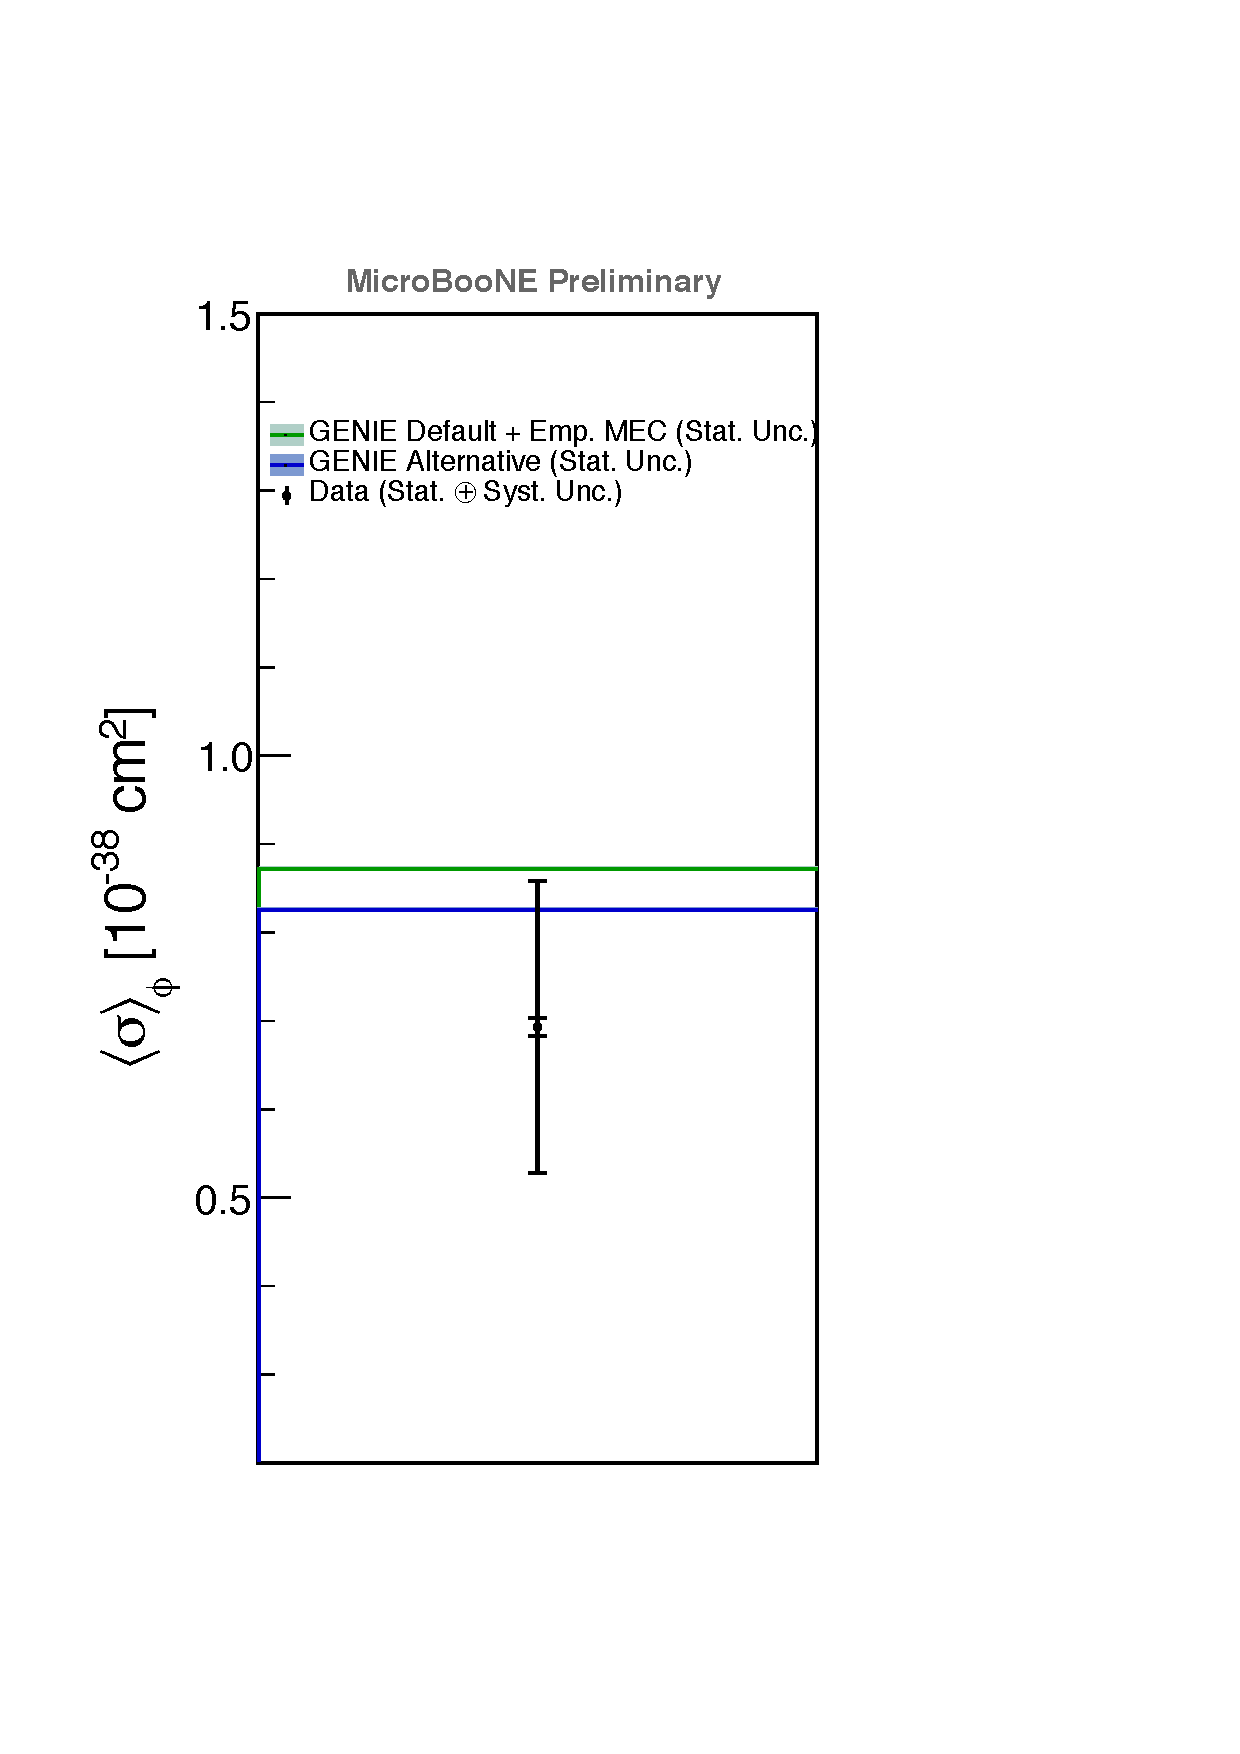
\includegraphics[width=.30\textwidth]{images/XSecFinal/onebin_xsec}
%\caption{$\nu_\mu$ \acrshort{cc} inclusive total cross section on argon. The \tuneone \acrshort{mc} prediction is shown in green, while the \tunethree prediction is shown in blue. The error bars show statistical and systematic uncertainties.}
%\label{fig:total_xsec_wsyst}
%\end{figure}

\begin{figure}[]
\centering
\subfloat[][]
   {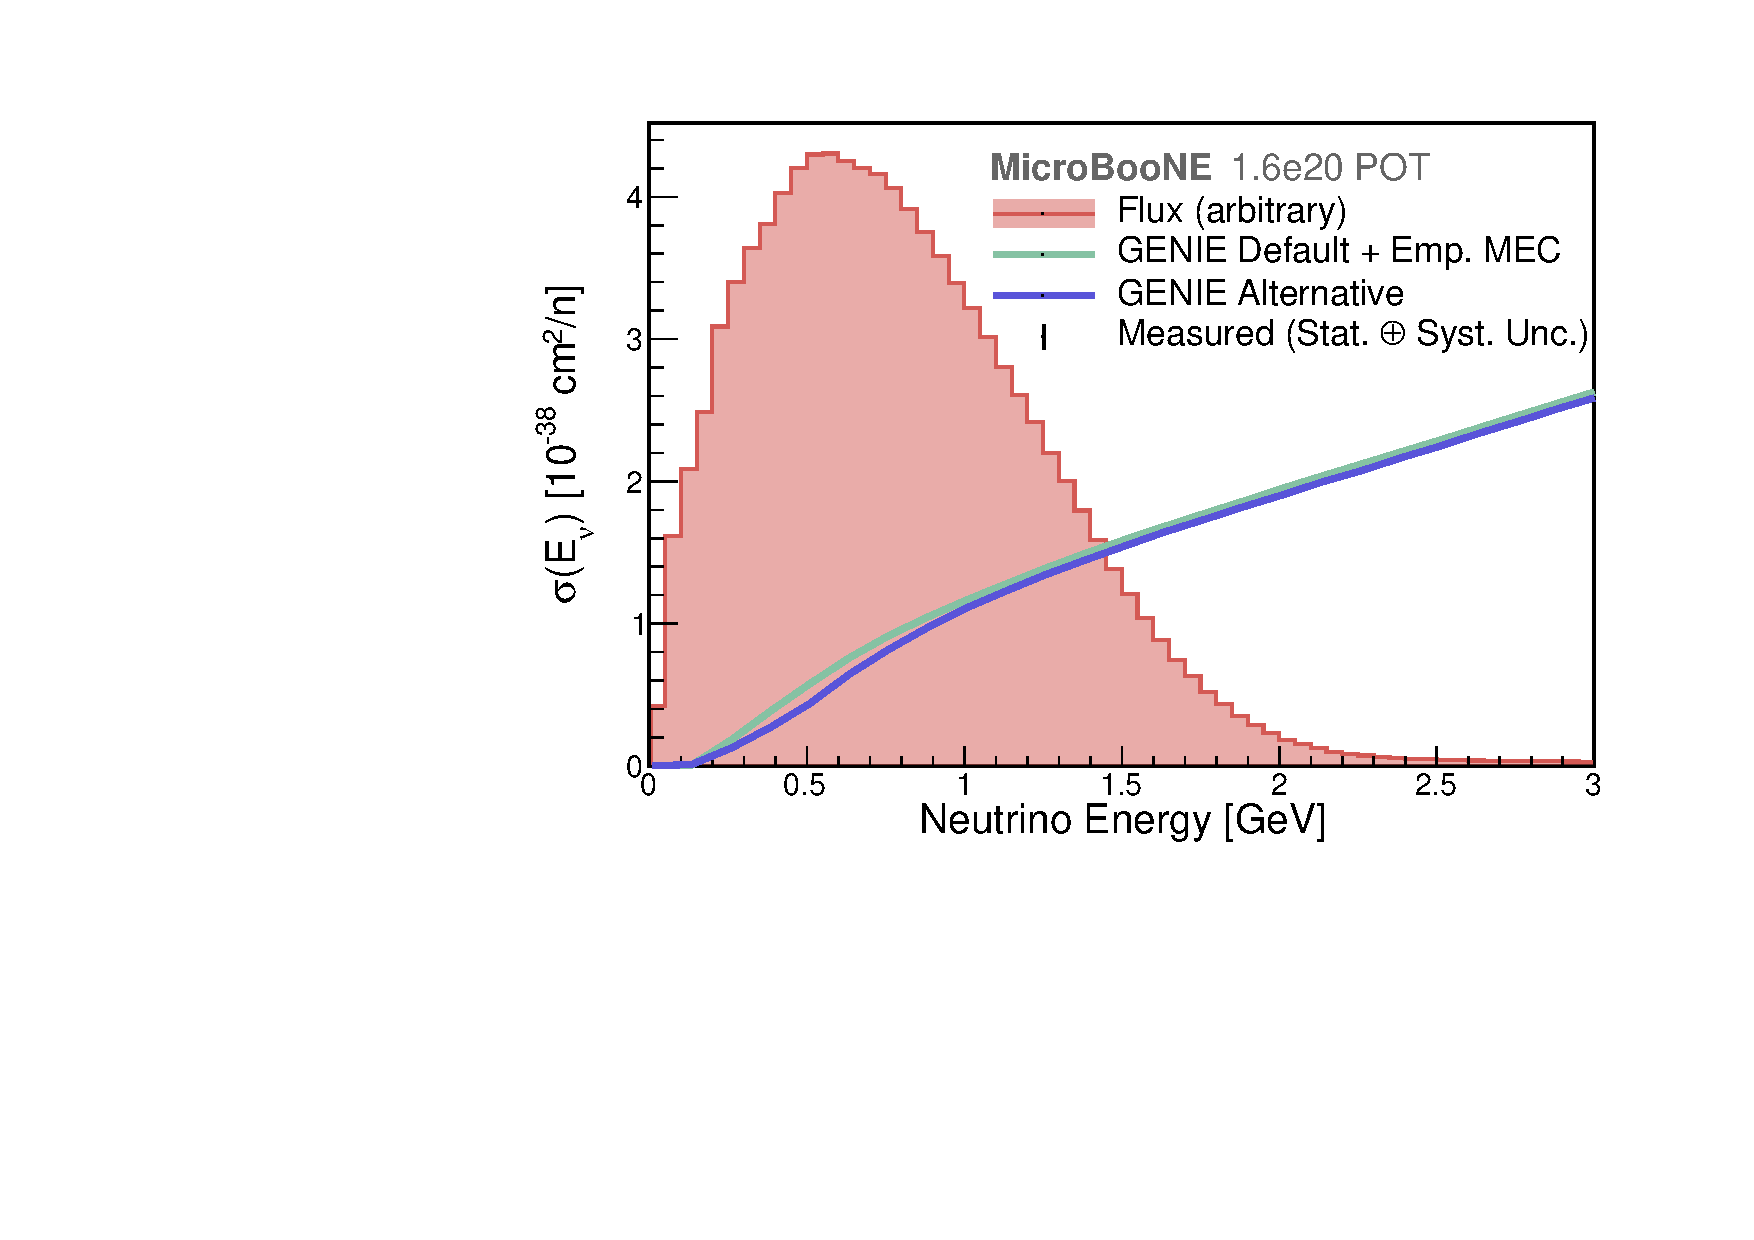
\includegraphics[width=.70\textwidth]{images/XSecFinal/flux_xsec_plot}
   \label{fig:flux_xsec_plot}}
\subfloat[][]
   {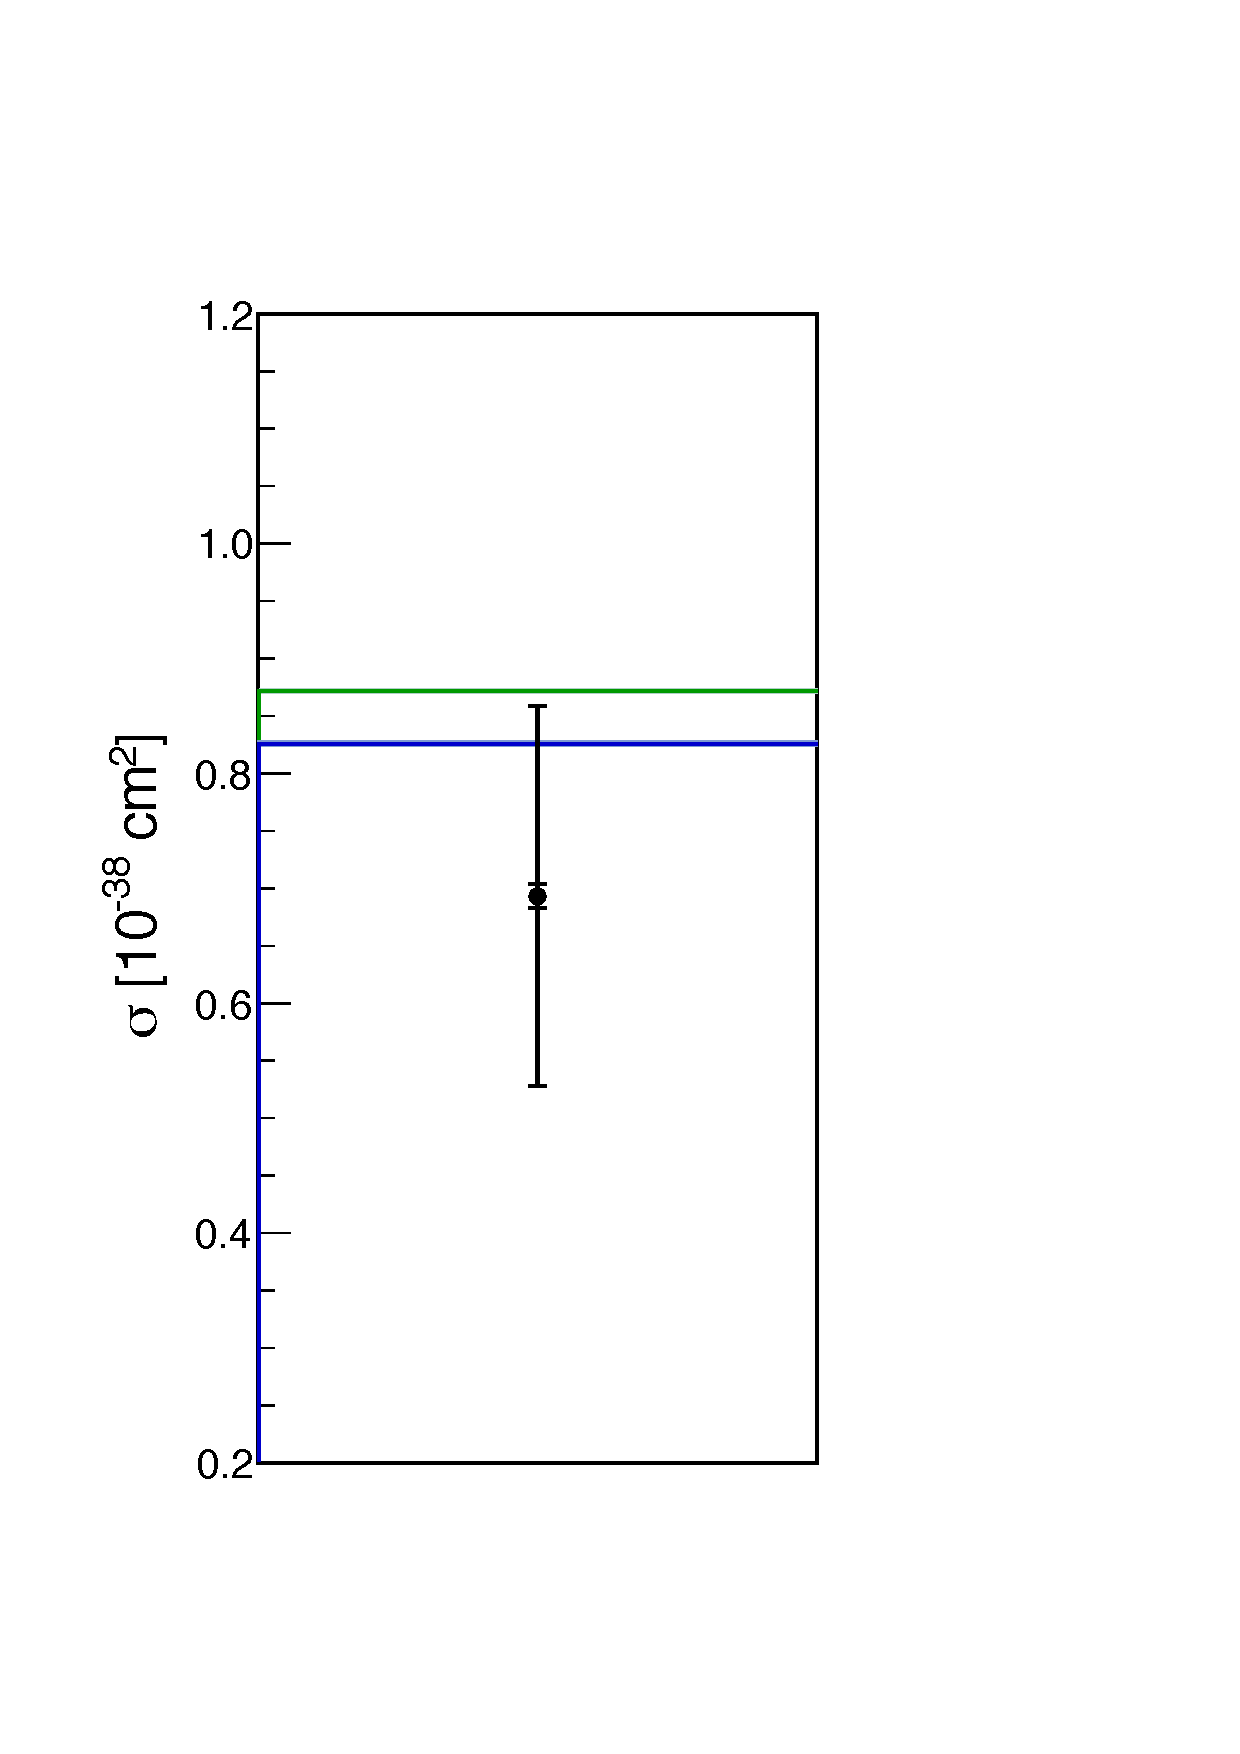
\includegraphics[width=.28\textwidth]{images/XSecFinal/onebin_xsec_simple}
   \label{fig:trkmom_xsec_tune3_wsyst}} \\
\caption[Total Cross Section (Stat. $\oplus$ Syst. Unc.)]{Predicted $\nu_\mu$ \acrshort{cc} inclusive  cross section on argon per nucleon $n$ as a function of neutrino energy~\protect\subref{fig:flux_xsec_plot}. The ``\tuneone'' \acrshort{mc} prediction is shown in green, while the ``\tunethree'' prediction is shown in blue. For comparison, the neutrino flux at MicroBooNE (with an arbitrary scale) is shown in red. The total measured cross section is shown in~\protect\subref{fig:trkmom_xsec_tune3_wsyst} with a black point. The inner vertical bars show statistical uncertainties, while the outer ones show the quadrature sum of the statistical and systematic uncertainties.}
\label{fig:total_xsec_wsyst}
\end{figure}



\begin{figure}[]
\centering
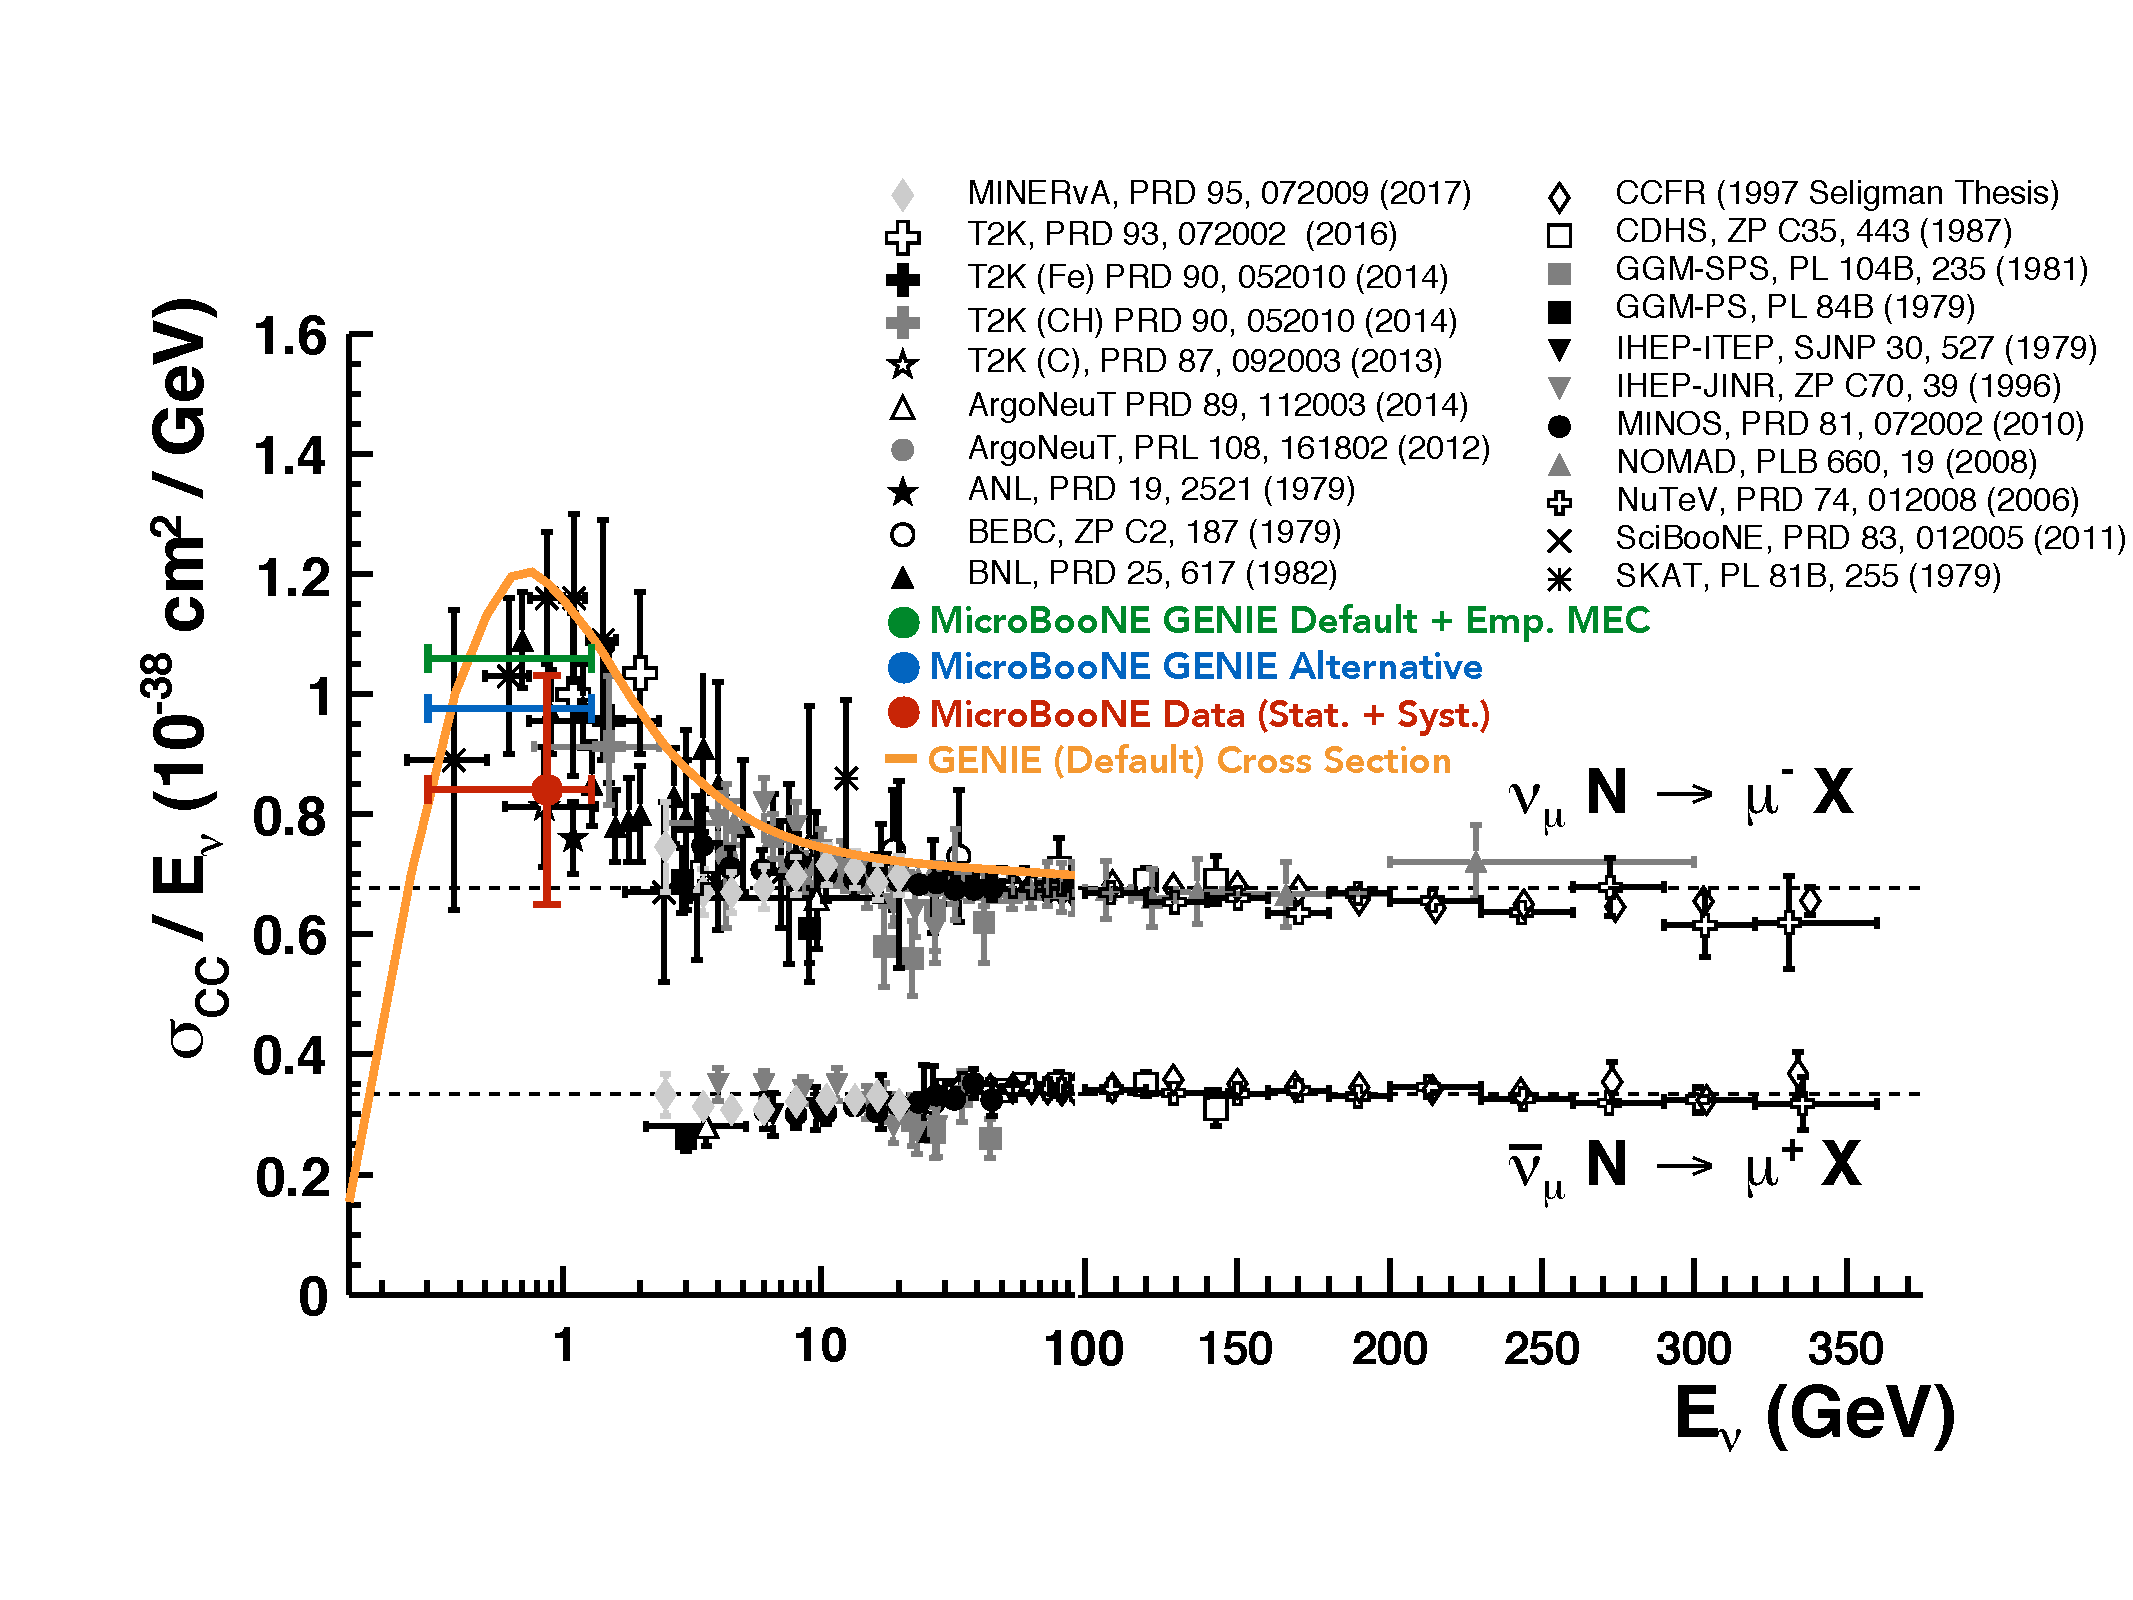
\includegraphics[width=.95\textwidth]{images/total_xsec_pdg_wsyst_2}
\caption[Total Cross Section (Stat. $\oplus$ Syst. Unc.) with Measurements from Different Experiments]{\acrshort{cc} inclusive measurements for $\nu_\mu$ and $\bar{\nu}_\mu$ from different experiments with different nuclear targets in black and grey. The coloured points represent the result and \acrshort{mc} predictions from this analysis. The green point shows the \acrshort{mc} extracted cross section according to the ``\tuneone'' configuration, the blue point according to the ``\tunethree'' configuration, and the red one shows the data extracted cross section. The vertical bars on the data cross section show the sum in quadrature of the statistical and systematic uncertainties. The orange curve shows the \g predicted cross section as a function of neutrino energy according to ``\tuneone''.}
\label{fig:total_xsec_pdg_wsyst}
\end{figure}


The single differential cross sections in muon momentum and angle are shown in Figure~\ref{fig:xsec_wsyst}. The uncertainties shown in this figure are the square root of the diagonal elements of the total covariance matrix in Equation~\eqref{eq:tot_cov}. The total covariance matrices are shown in Figure~\ref{fig:xsec_tot_correlation_single}. 

The double-differential cross section in muon momentum and angle is shown in Figure~\ref{fig:3d_xsec} and in Figure~\ref{fig:trkcostheta_trkmumom__xsec_anglesplit} for different muon angle bins. The total covariance matrix for the double-differential is shown in Figure~\ref{fig:xsec_tot_correlation}. 

Tabulated values for the measured cross sections are reported in Appendix~\ref{ch:xsec_values}.

\begin{figure}[]
%\begin{adjustwidth}{-1.3cm}{-1cm}
\centering
\subfloat[][]
   {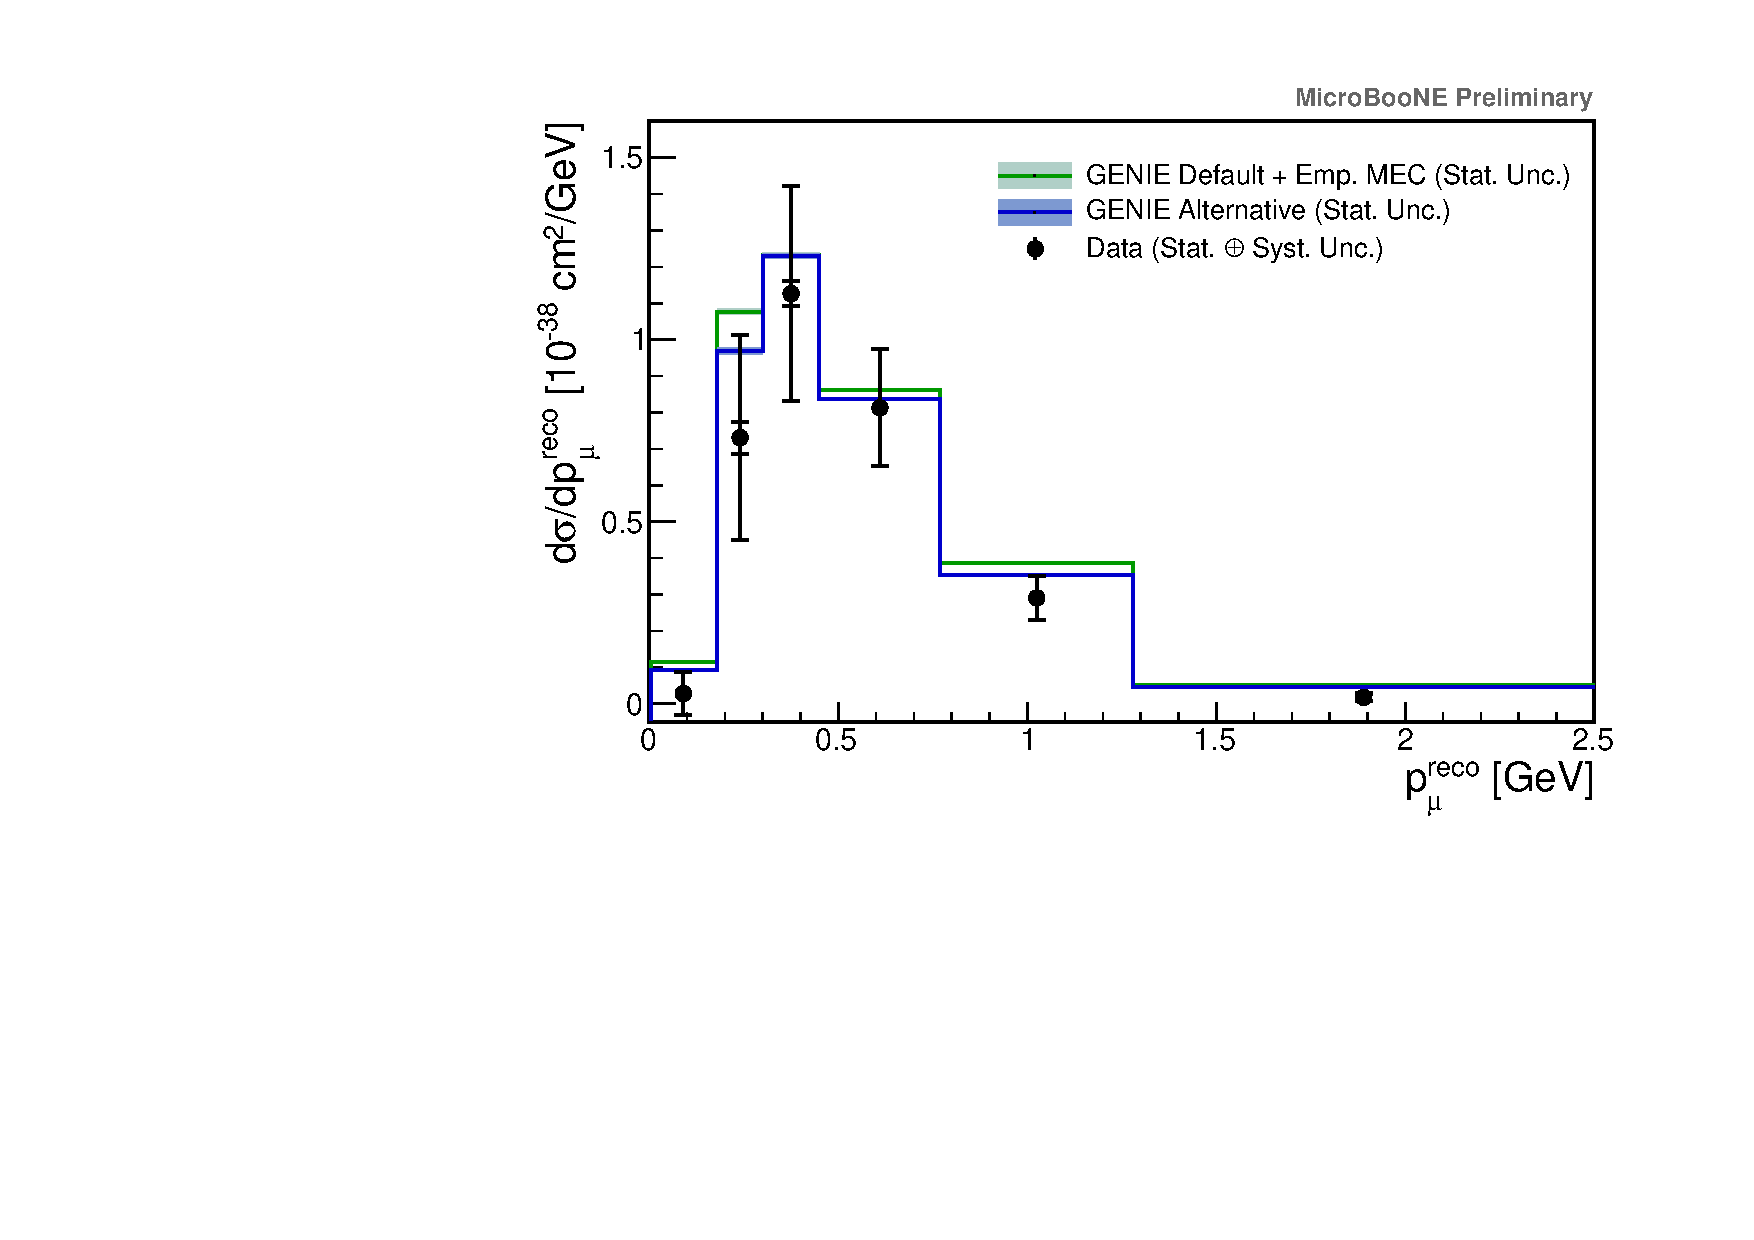
\includegraphics[width=.75\textwidth]{images/XSecFinal/trkmom_xsec}
   \label{fig:trkmom_xsec_tune1_wsyst}}\\
\subfloat[][]
   {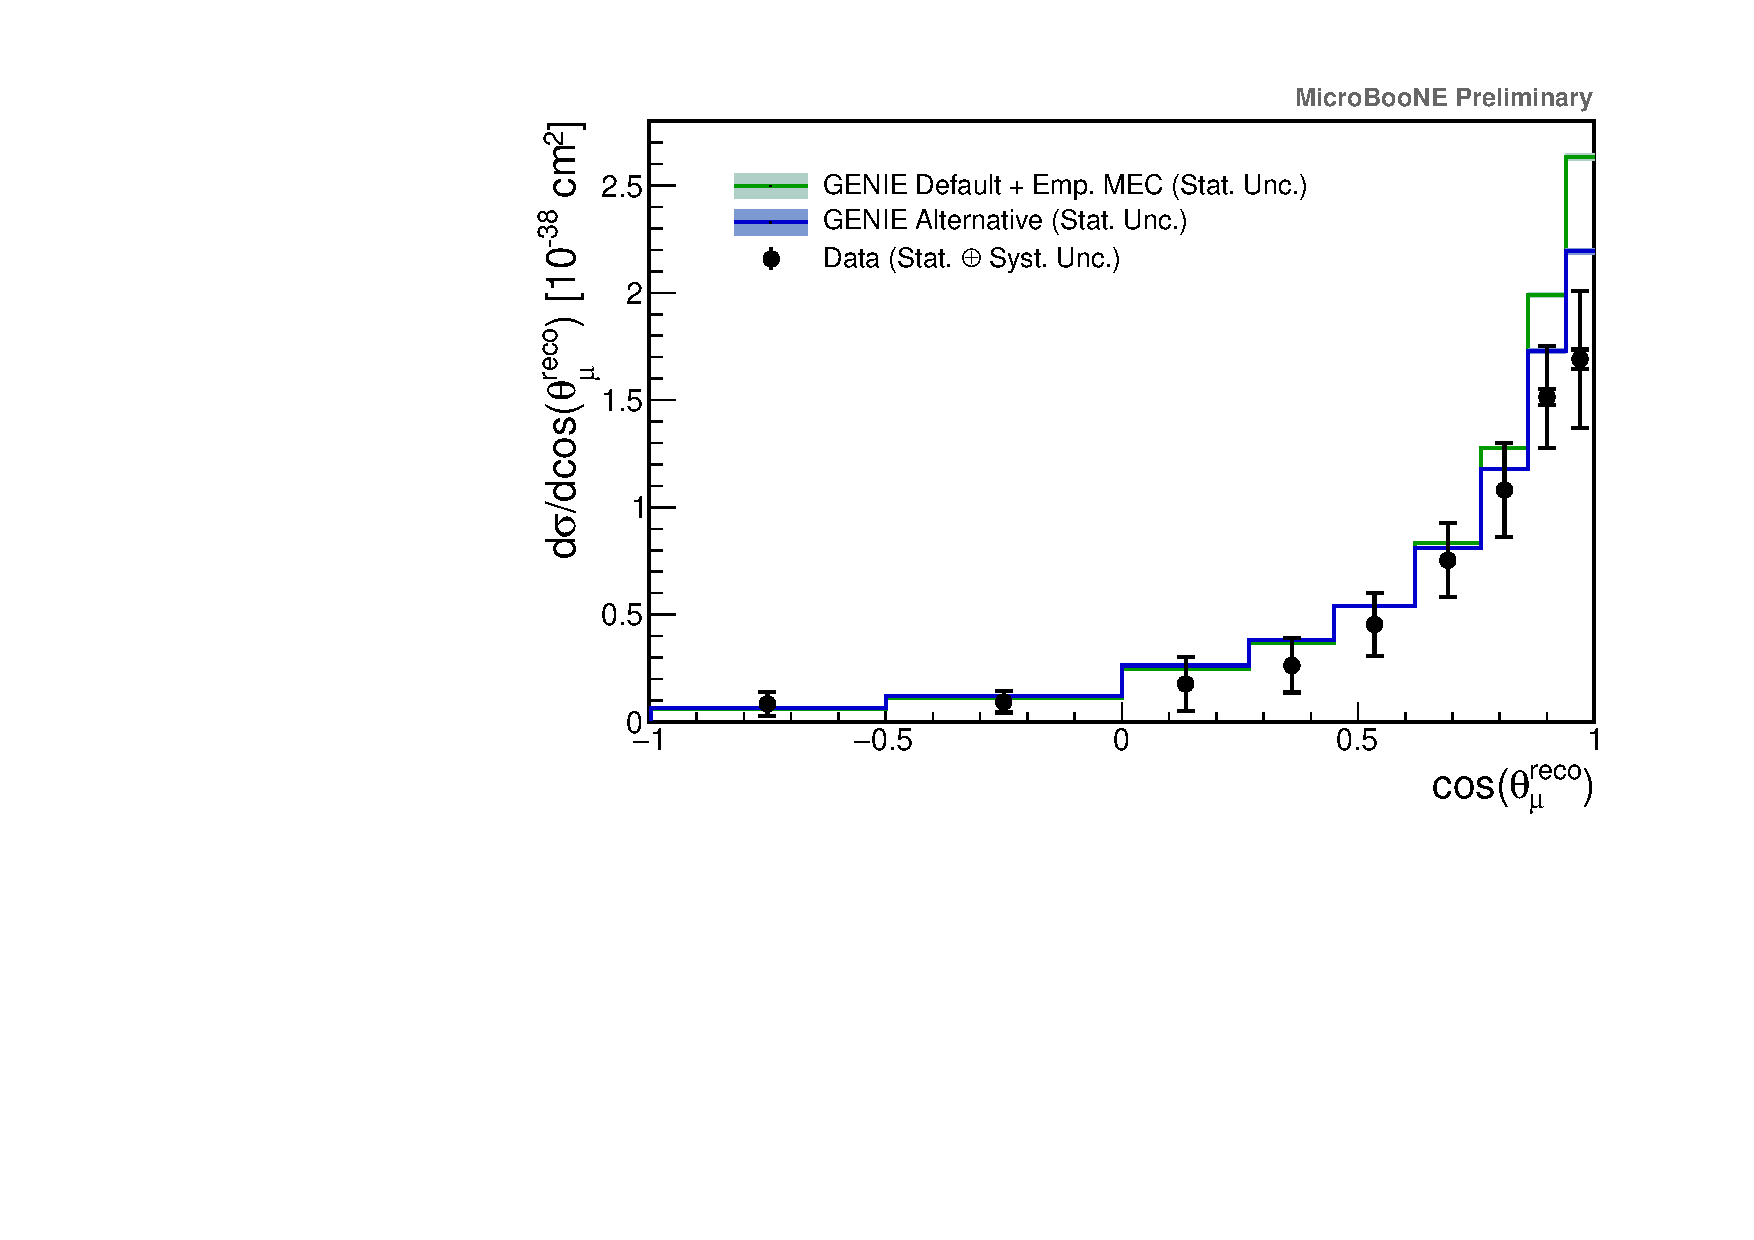
\includegraphics[width=.75\textwidth]{images/XSecFinal/trkcostheta_xsec}
   \label{fig:trkcostheta_xsec}} \\
\caption[Single-Differential Cross Sections (Stat. $\oplus$ Syst. Unc.)]{$\nu_\mu$ \acrshort{cc} inclusive single-differential cross section on argon per nucleon as a function of the reconstructed muon momentum~\protect\subref{fig:trkmom_xsec_tune1_wsyst} and cosine of the muon polar angle~\protect\subref{fig:trkcostheta_xsec}. The data (black) is compared to the default \g prediction (green) and the alternative \g prediction (blue), as described in the text.  The inner vertical bars show statistical uncertainties, while the outer ones show the quadrature sum of the statistical and systematic uncertainties.}
\label{fig:xsec_wsyst}
%\end{adjustwidth}
\end{figure}

\begin{figure}[]
\begin{adjustwidth}{-1.3cm}{-1cm}
\centering
\subfloat[][Covariance matrix, $p_\mu$ bins.]
   {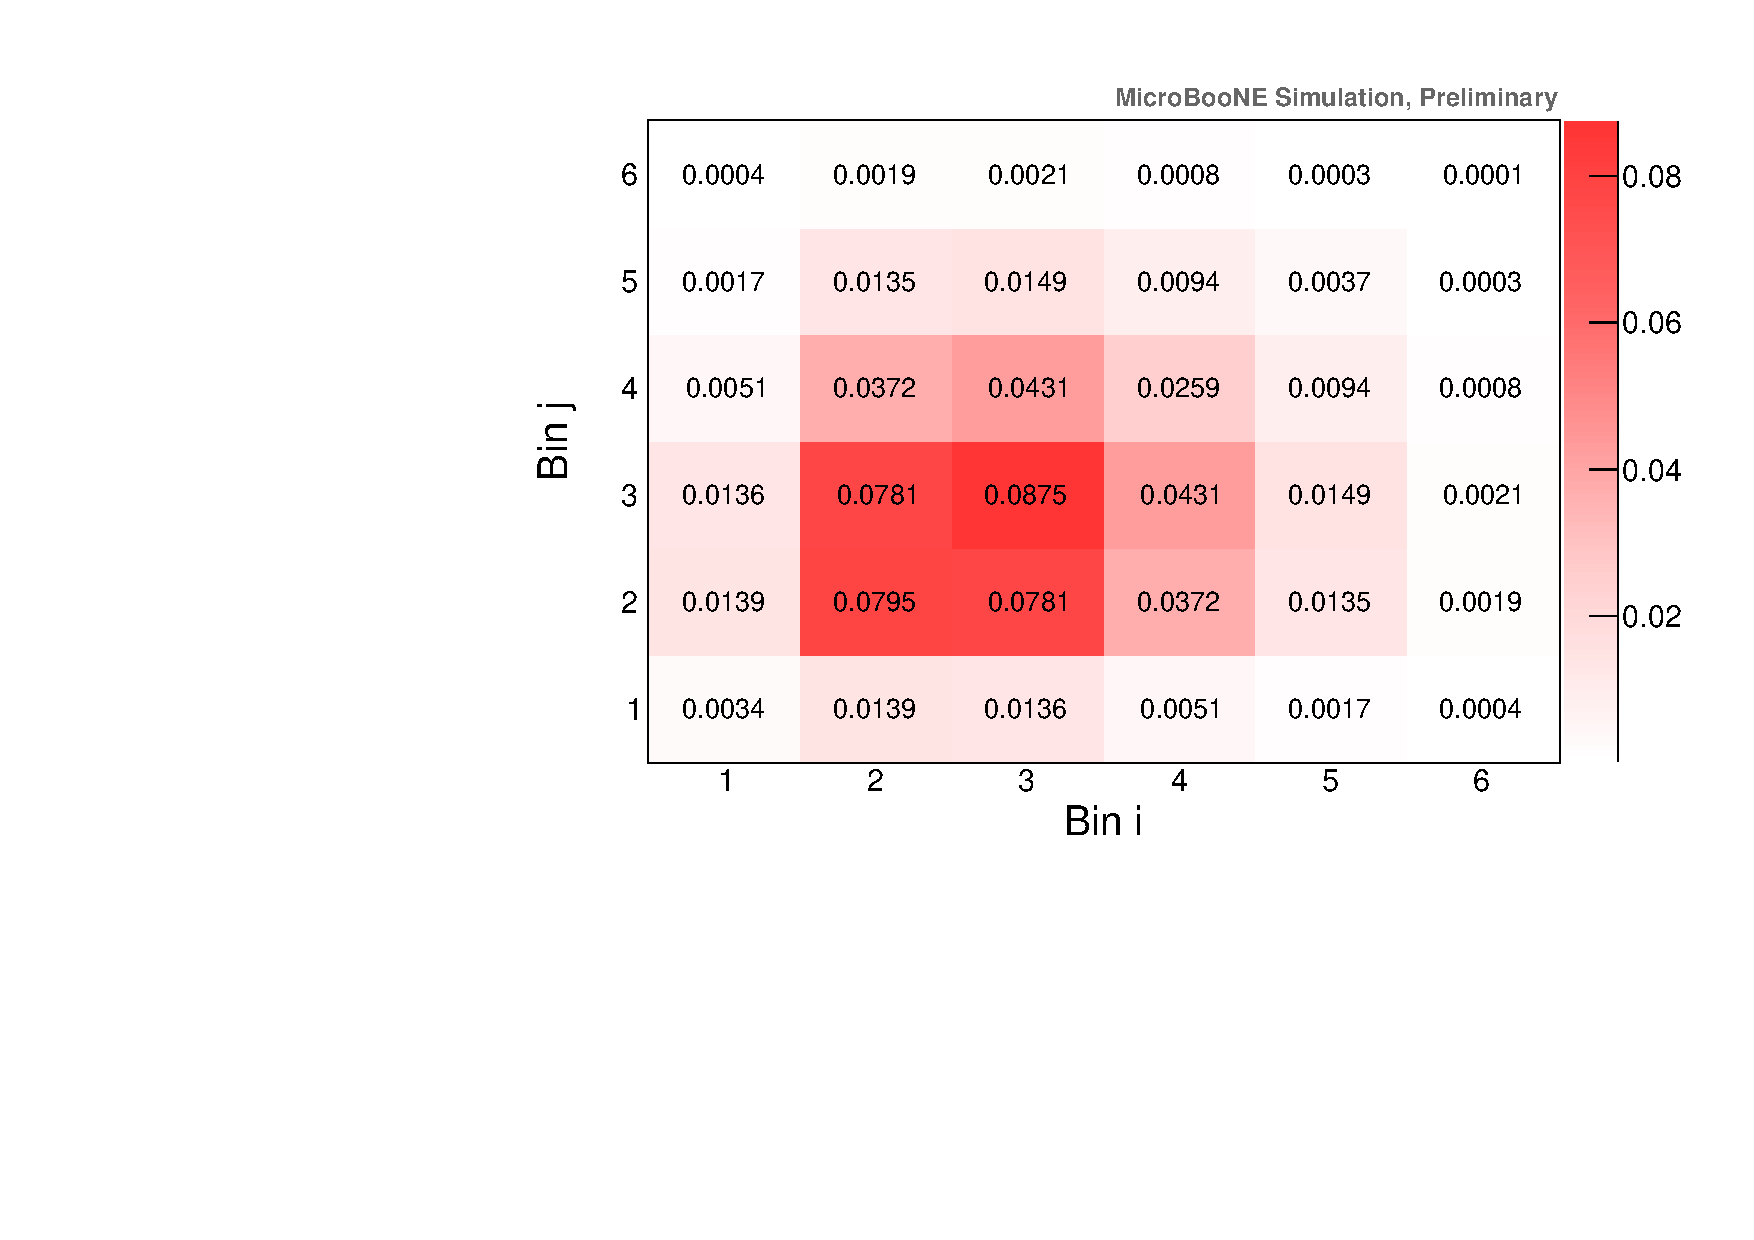
\includegraphics[width=.45\textwidth]{images/XSecFinal/trkmom_tot_covariance}
   \label{fig:trkmom_tot_covariance}} \quad
\subfloat[][Covariance matrix, $\cos\theta_\mu$ bins.]
   {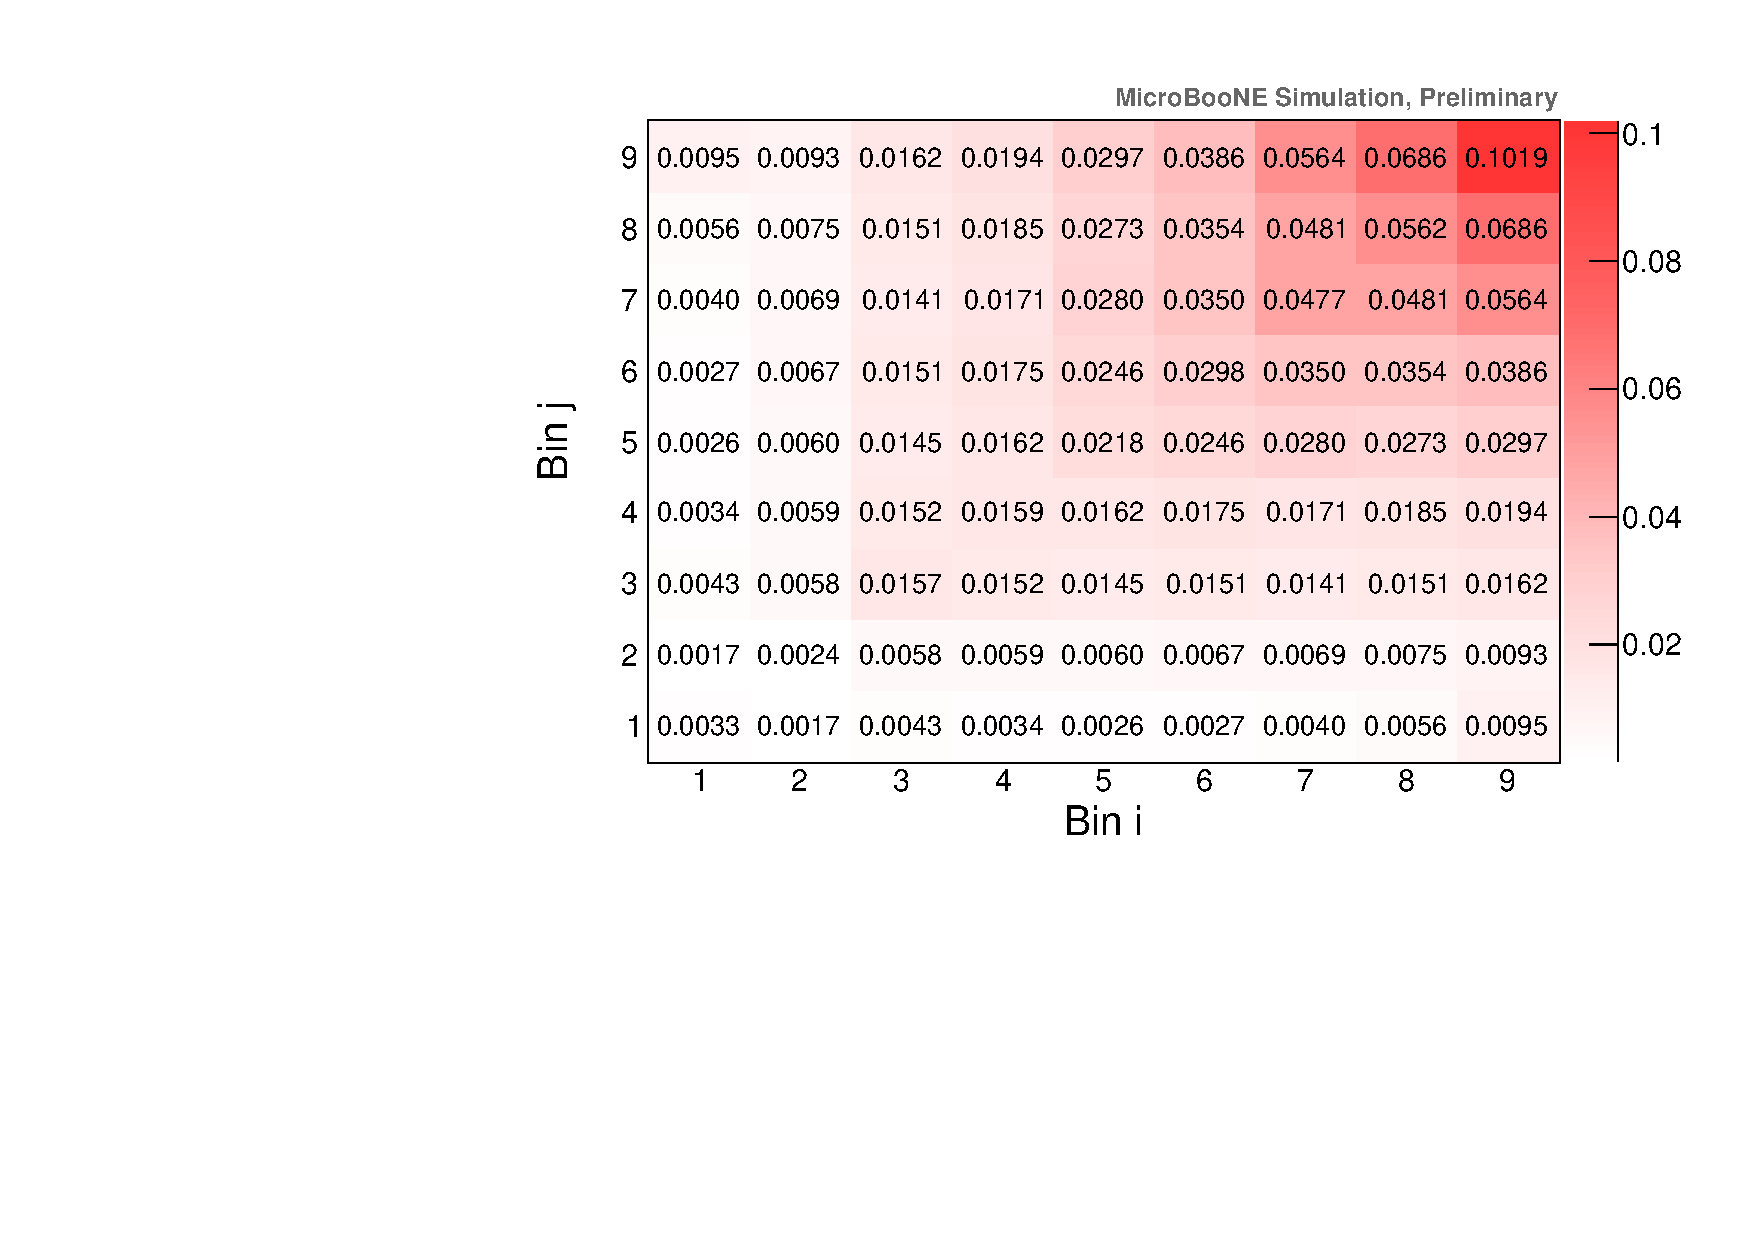
\includegraphics[width=.45\textwidth]{images/XSecFinal/trkcostheta_tot_covariance}
   \label{fig:trkcostheta_tot_covariance}} \\
\subfloat[][Fractional covariance matrix, $p_\mu$ bins.]
   {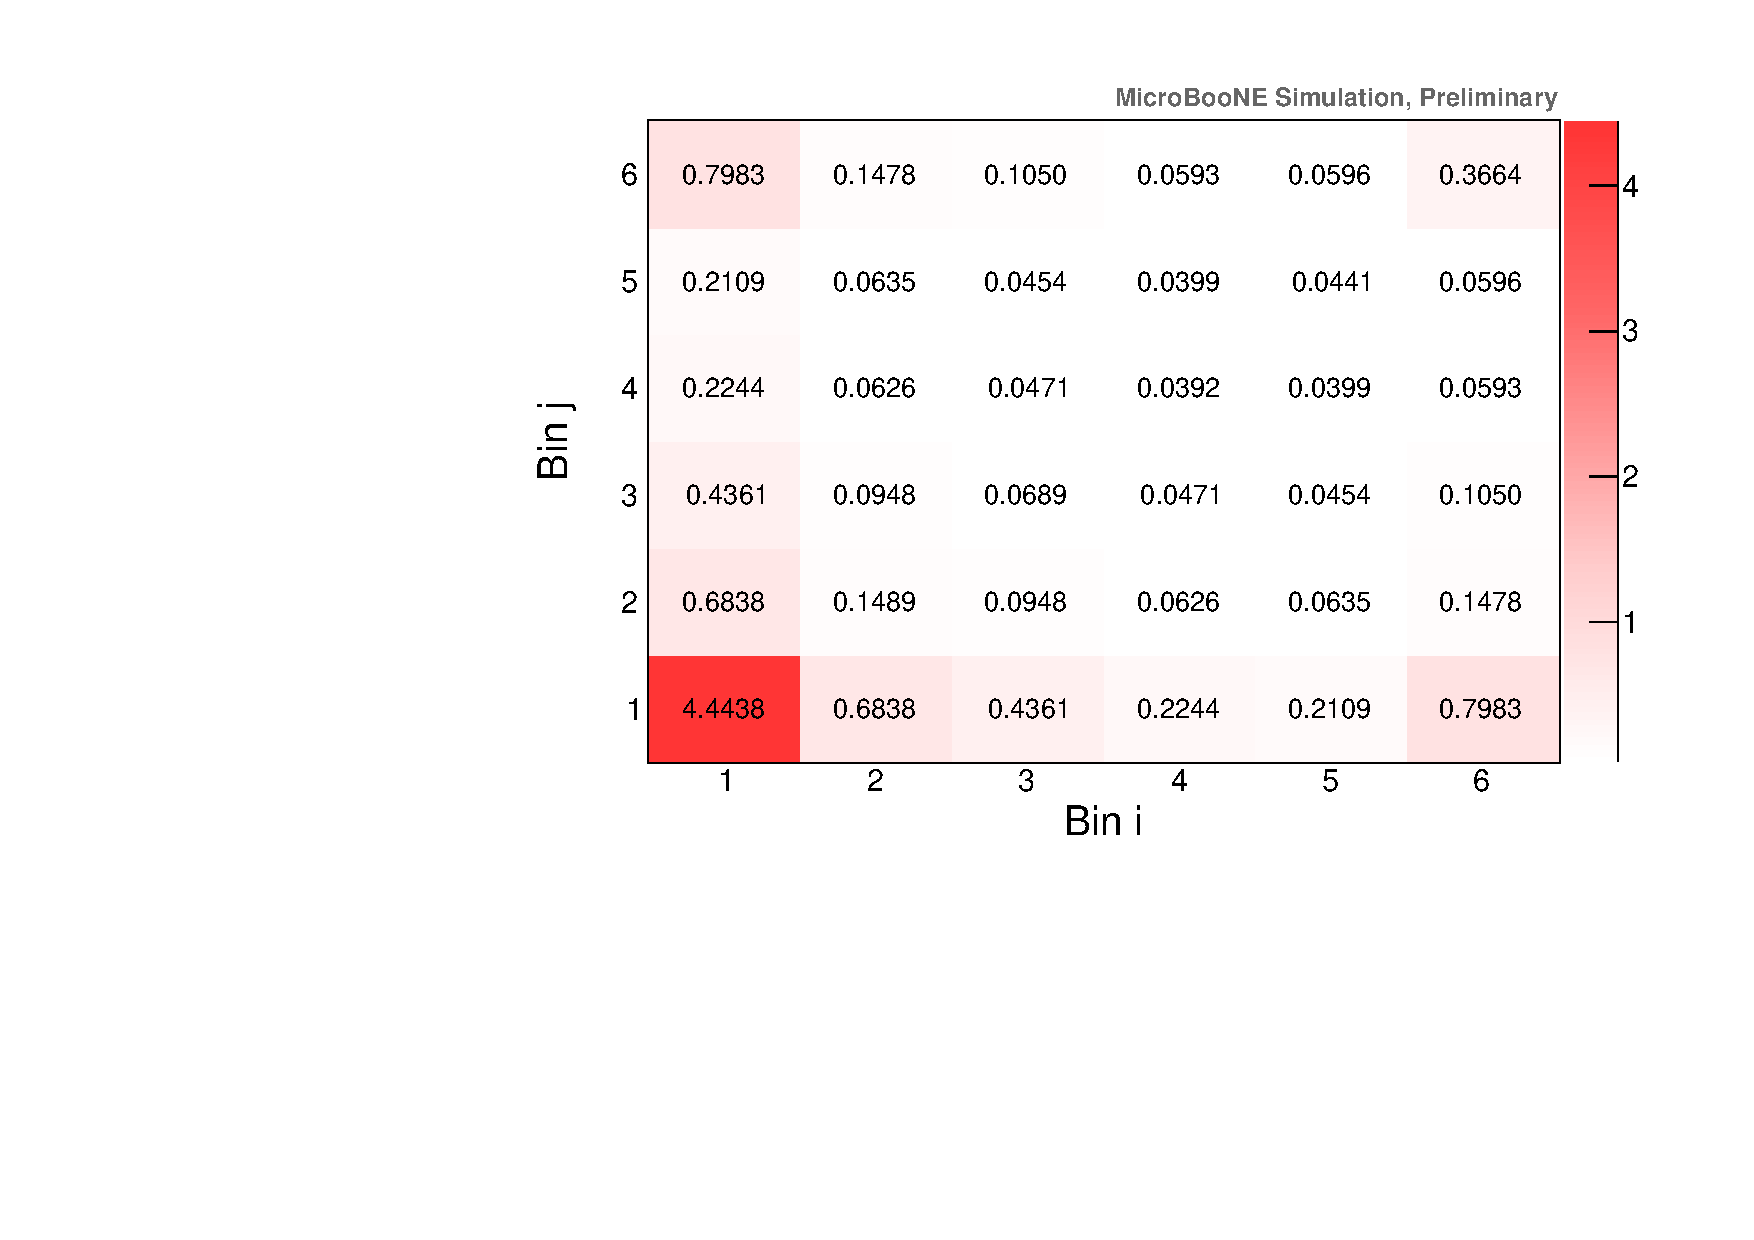
\includegraphics[width=.45\textwidth]{images/XSecFinal/trkmom_tot_fractional_covariance}
   \label{fig:trkmom_tot_fractional_covariance}} \quad
\subfloat[][Fractional covariance matrix, $\cos\theta_\mu$ bins.]
   {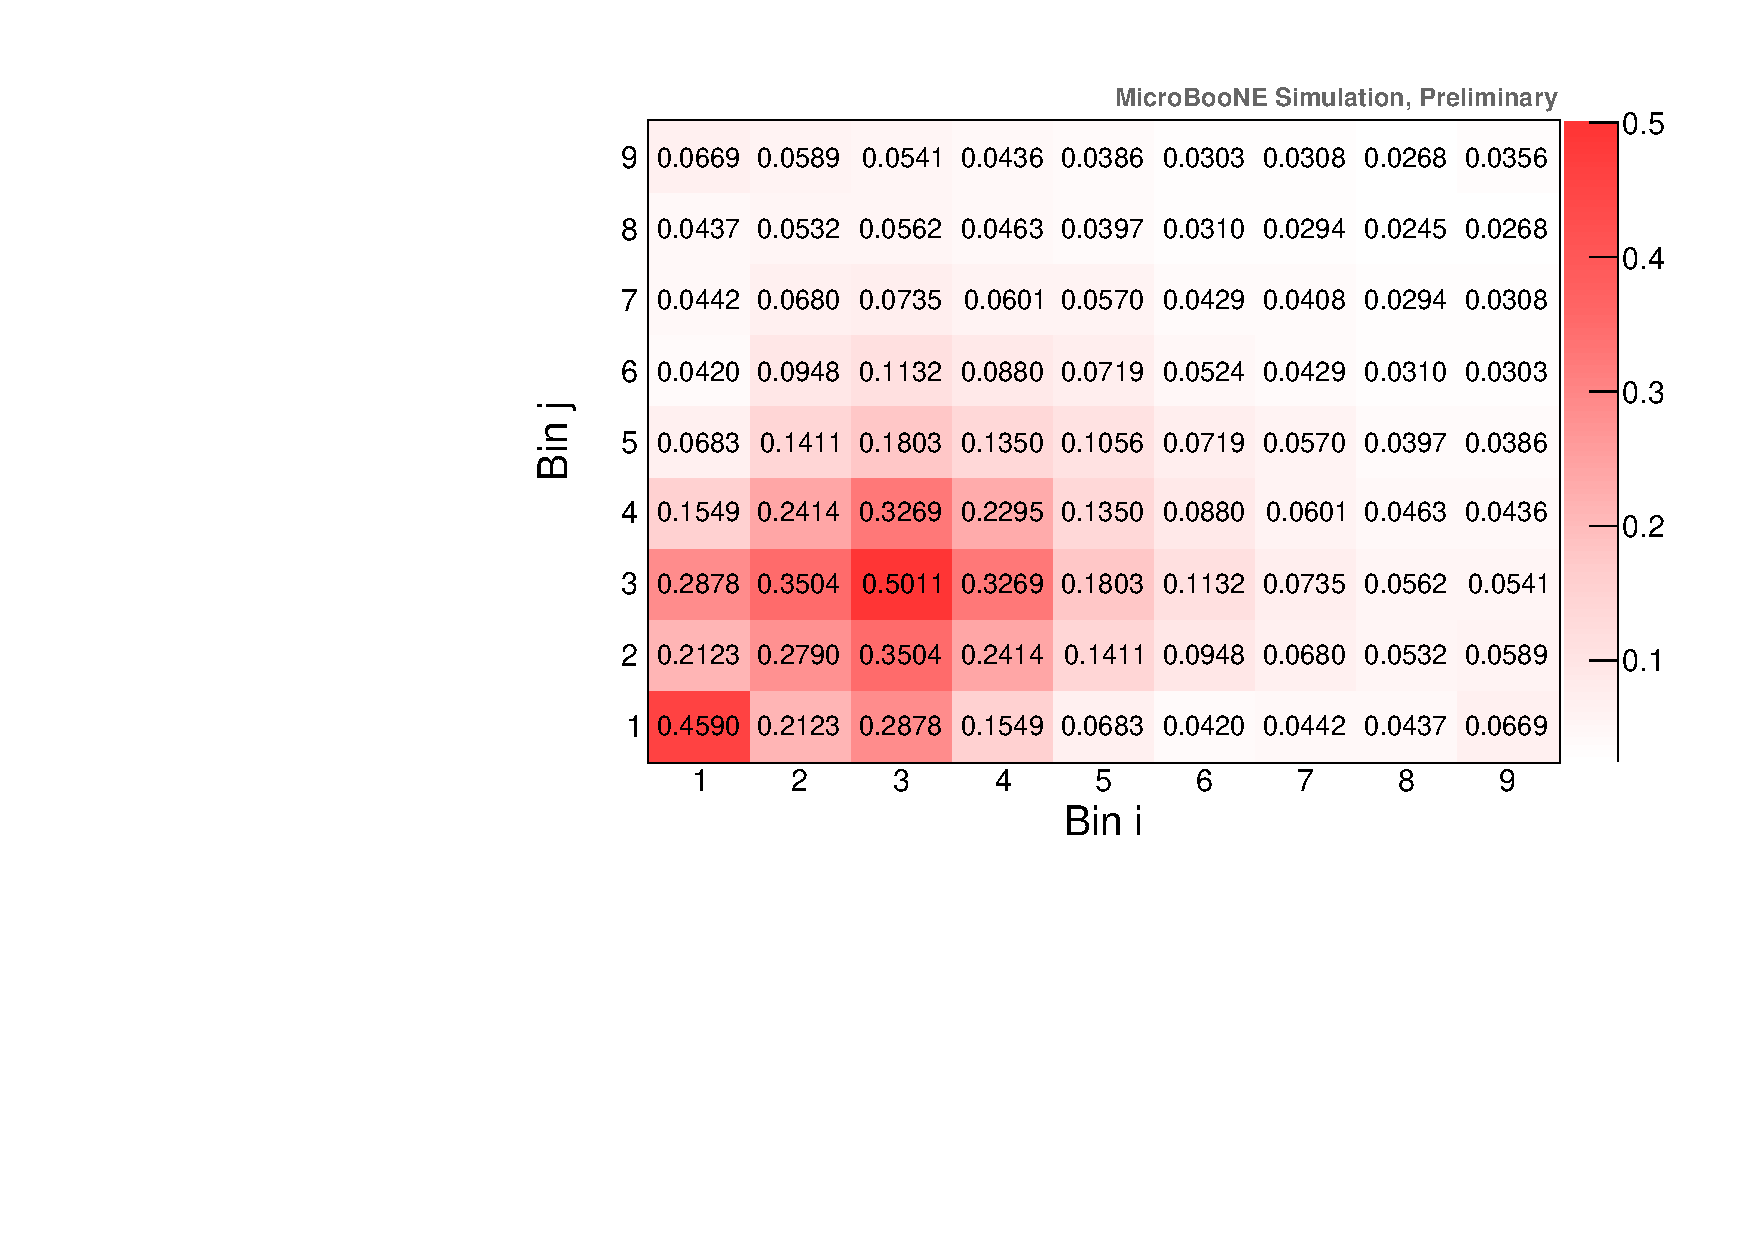
\includegraphics[width=.45\textwidth]{images/XSecFinal/trkcostheta_tot_fractional_covariance}
   \label{fig:trkcostheta_tot_fractional_covariance}} \\
\subfloat[][Correlation matrix, $p_\mu$ bins.]
   {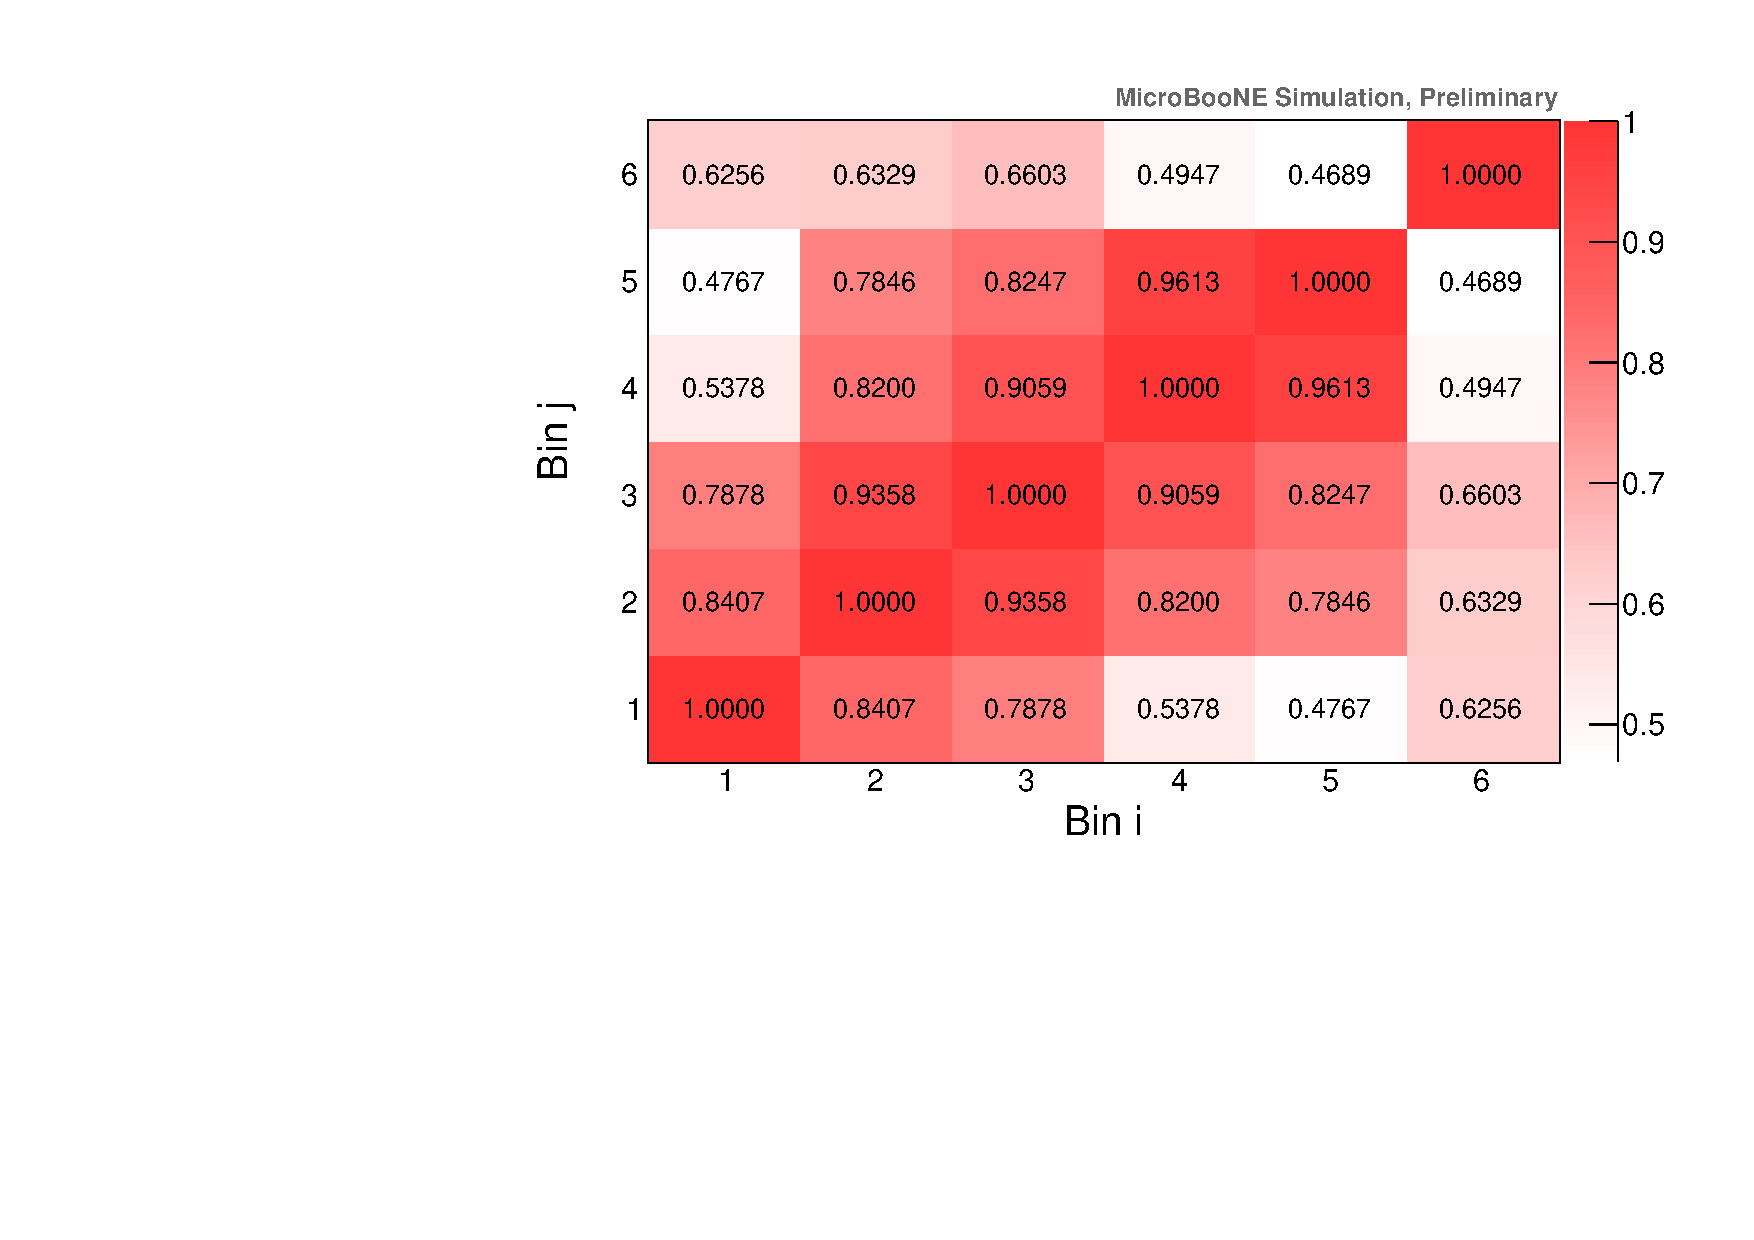
\includegraphics[width=.45\textwidth]{images/XSecFinal/trkmom_tot_correlation}
   \label{fig:trkmom_tot_correlation}} \quad
\subfloat[][Correlation matrix, $\cos\theta_\mu$ bins.]
   {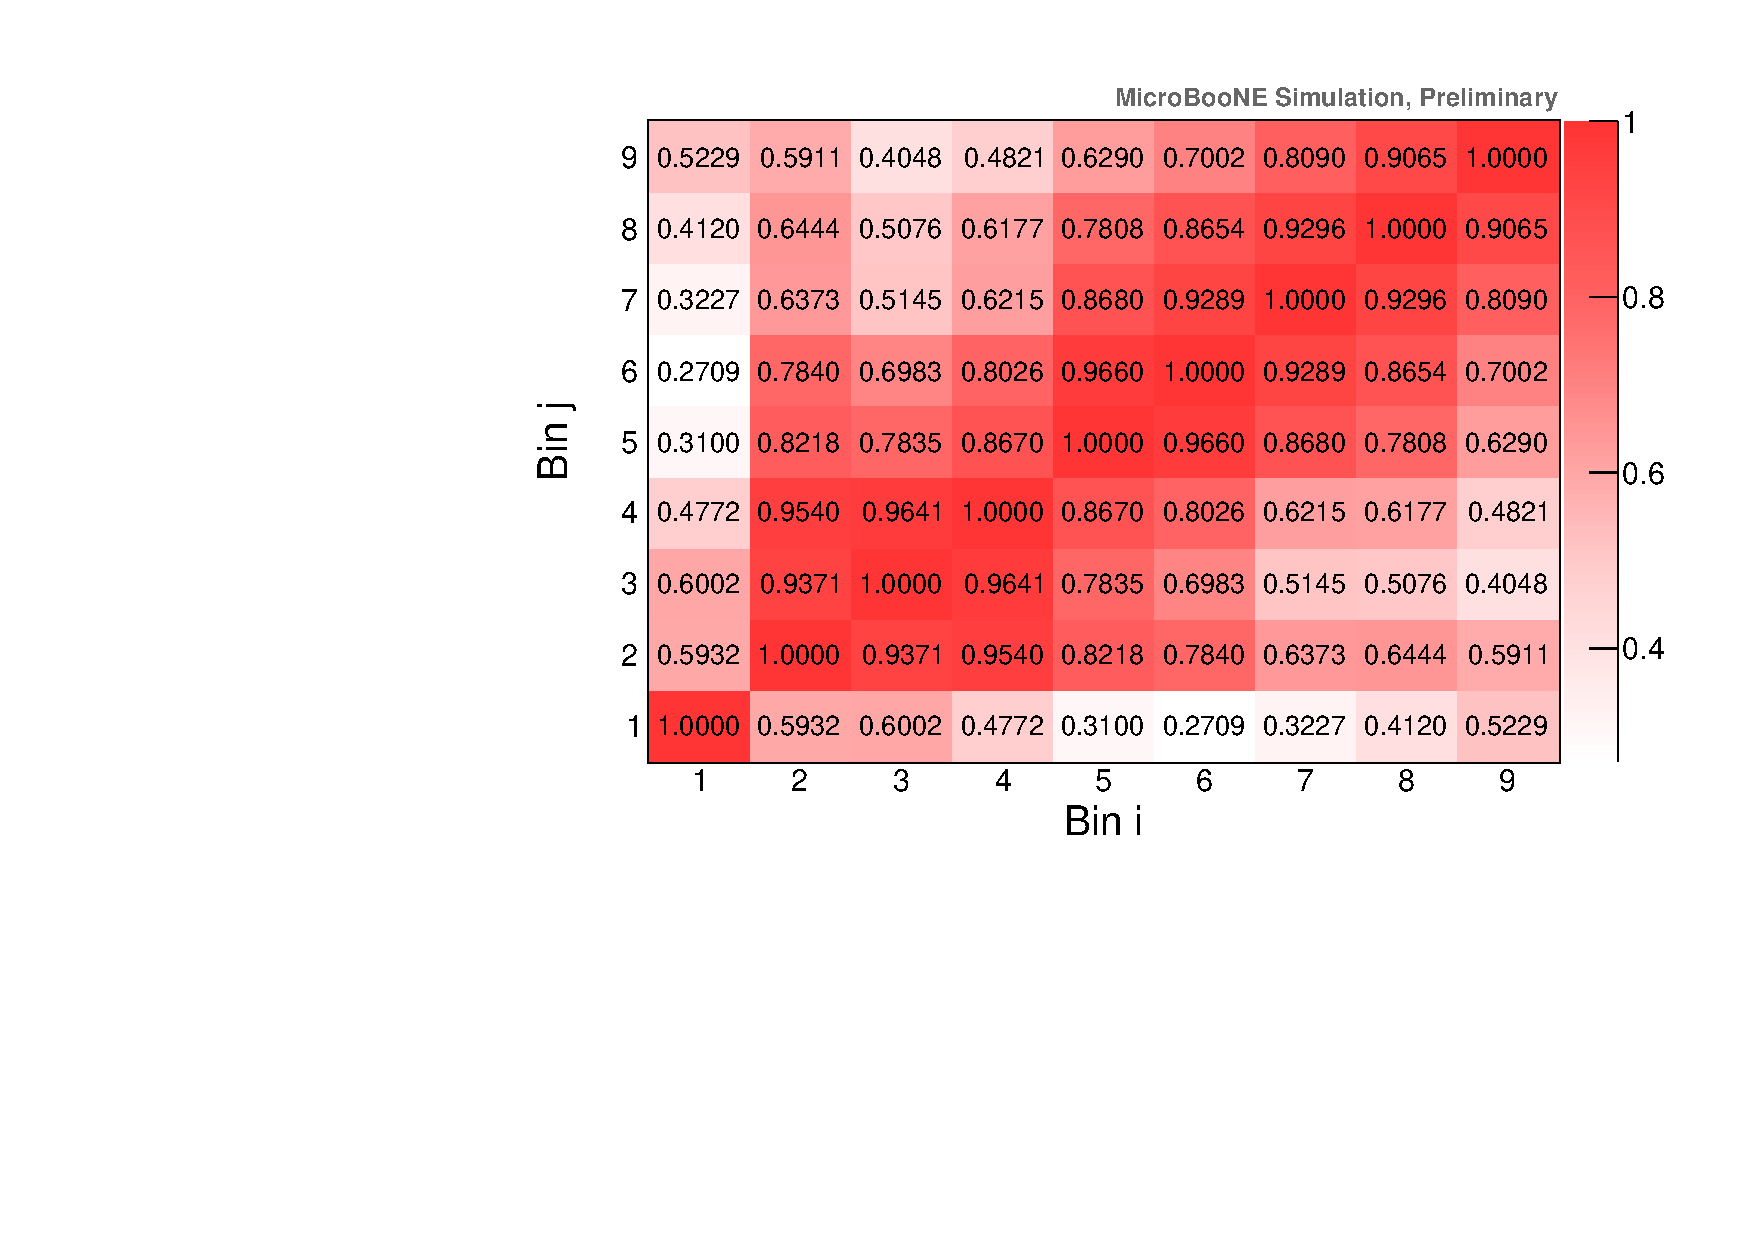
\includegraphics[width=.45\textwidth]{images/XSecFinal/trkcostheta_tot_correlation}
   \label{fig:trkcostheta_tot_correlation}} \\
\caption[Single-Differential Cross Sections - Total Covariance Matrices]{Total covariance (\protect\subref{fig:trkmom_tot_covariance},~\protect\subref{fig:trkcostheta_tot_covariance}), fractional covariance (\protect\subref{fig:trkmom_tot_fractional_covariance},~\protect\subref{fig:trkcostheta_tot_fractional_covariance}) and correlation (\protect\subref{fig:trkmom_tot_correlation},~\protect\subref{fig:trkcostheta_tot_correlation}) matrices for the $p_\mu$ and $\cos\theta_\mu$ bins. For the bin definition, see Section~\ref{sec:binning}.}
\label{fig:xsec_tot_correlation_single}
\end{adjustwidth}
\end{figure}

\begin{figure}[]
\centering
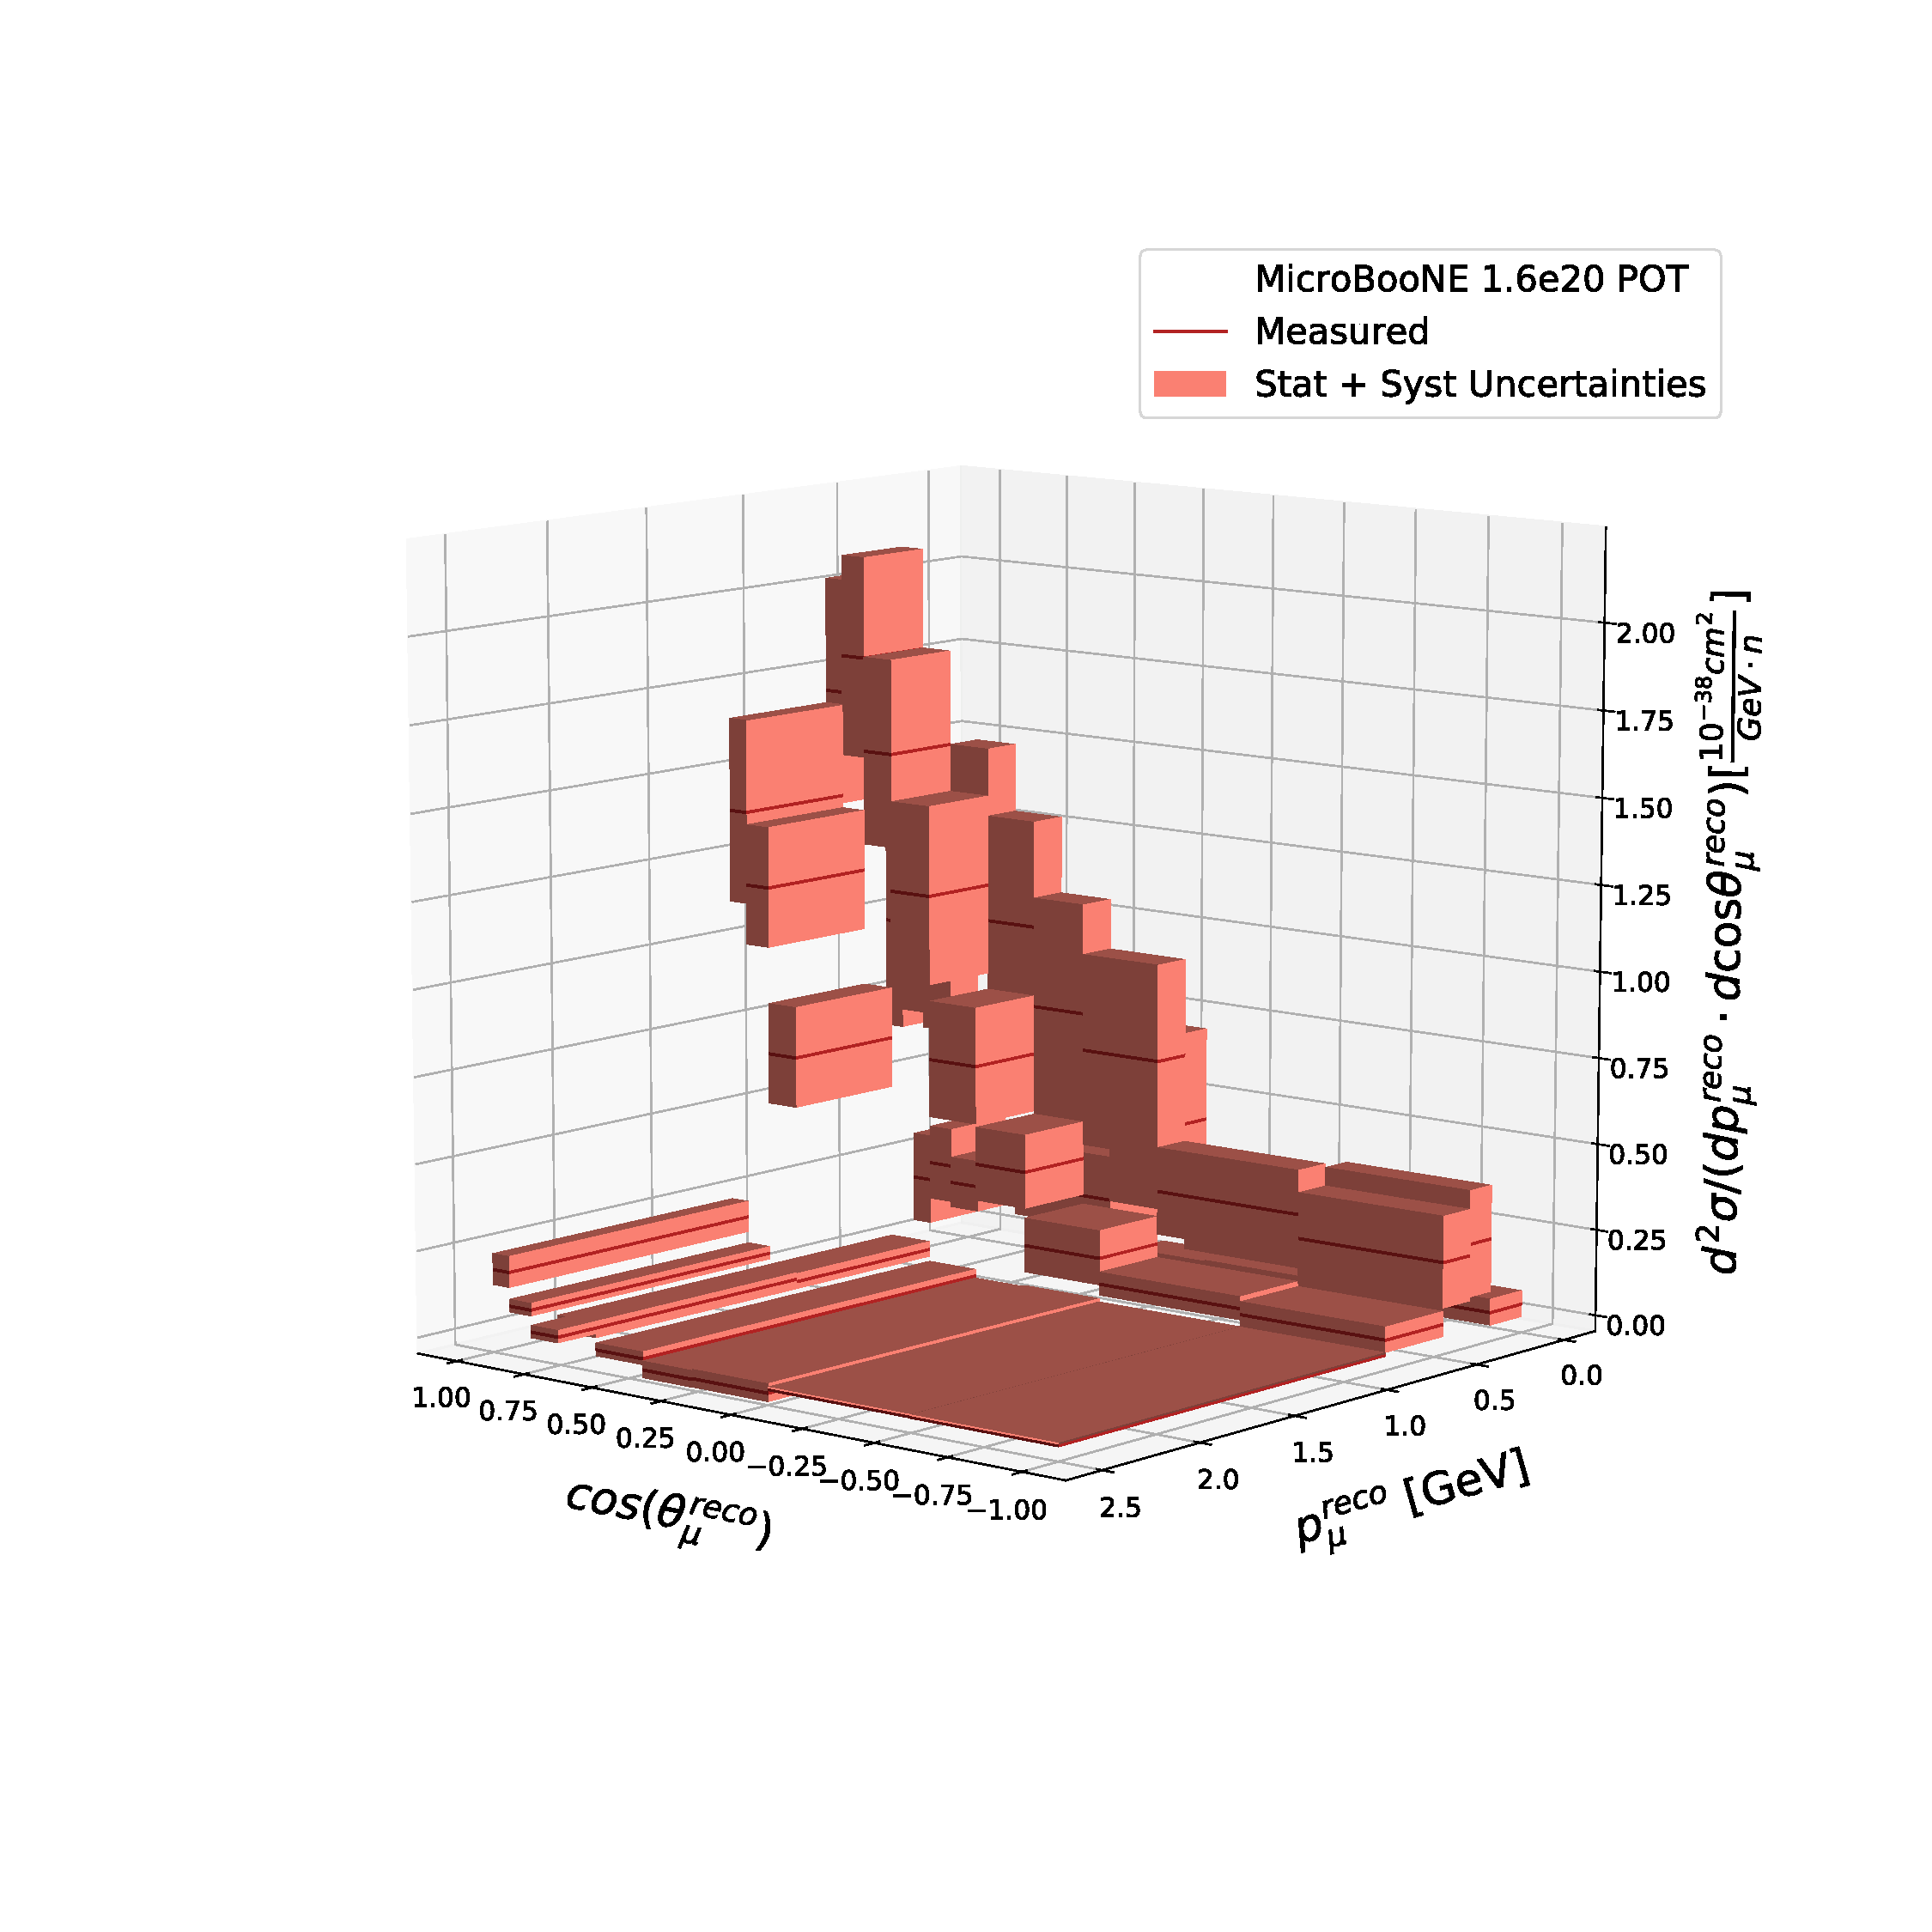
\includegraphics[width=1.0\textwidth]{images/XSecFinal/3d_xsec} %trkcostheta_trkmumom__xsec_anglesplit
\caption[Double-Differential Cross Section (Stat. $\oplus$ Syst. Unc.)]{$\nu_\mu$ \acrshort{cc} inclusive double-differential cross section on argon per nucleon as a function of the reconstructed muon momentum $p_\mu$ and cosine of the reconstructed muon polar angle $\cos\theta_\mu$ (angle with respect to the incoming neutrino direction).}
\label{fig:3d_xsec}
\end{figure}

\begin{figure}[]
\centering
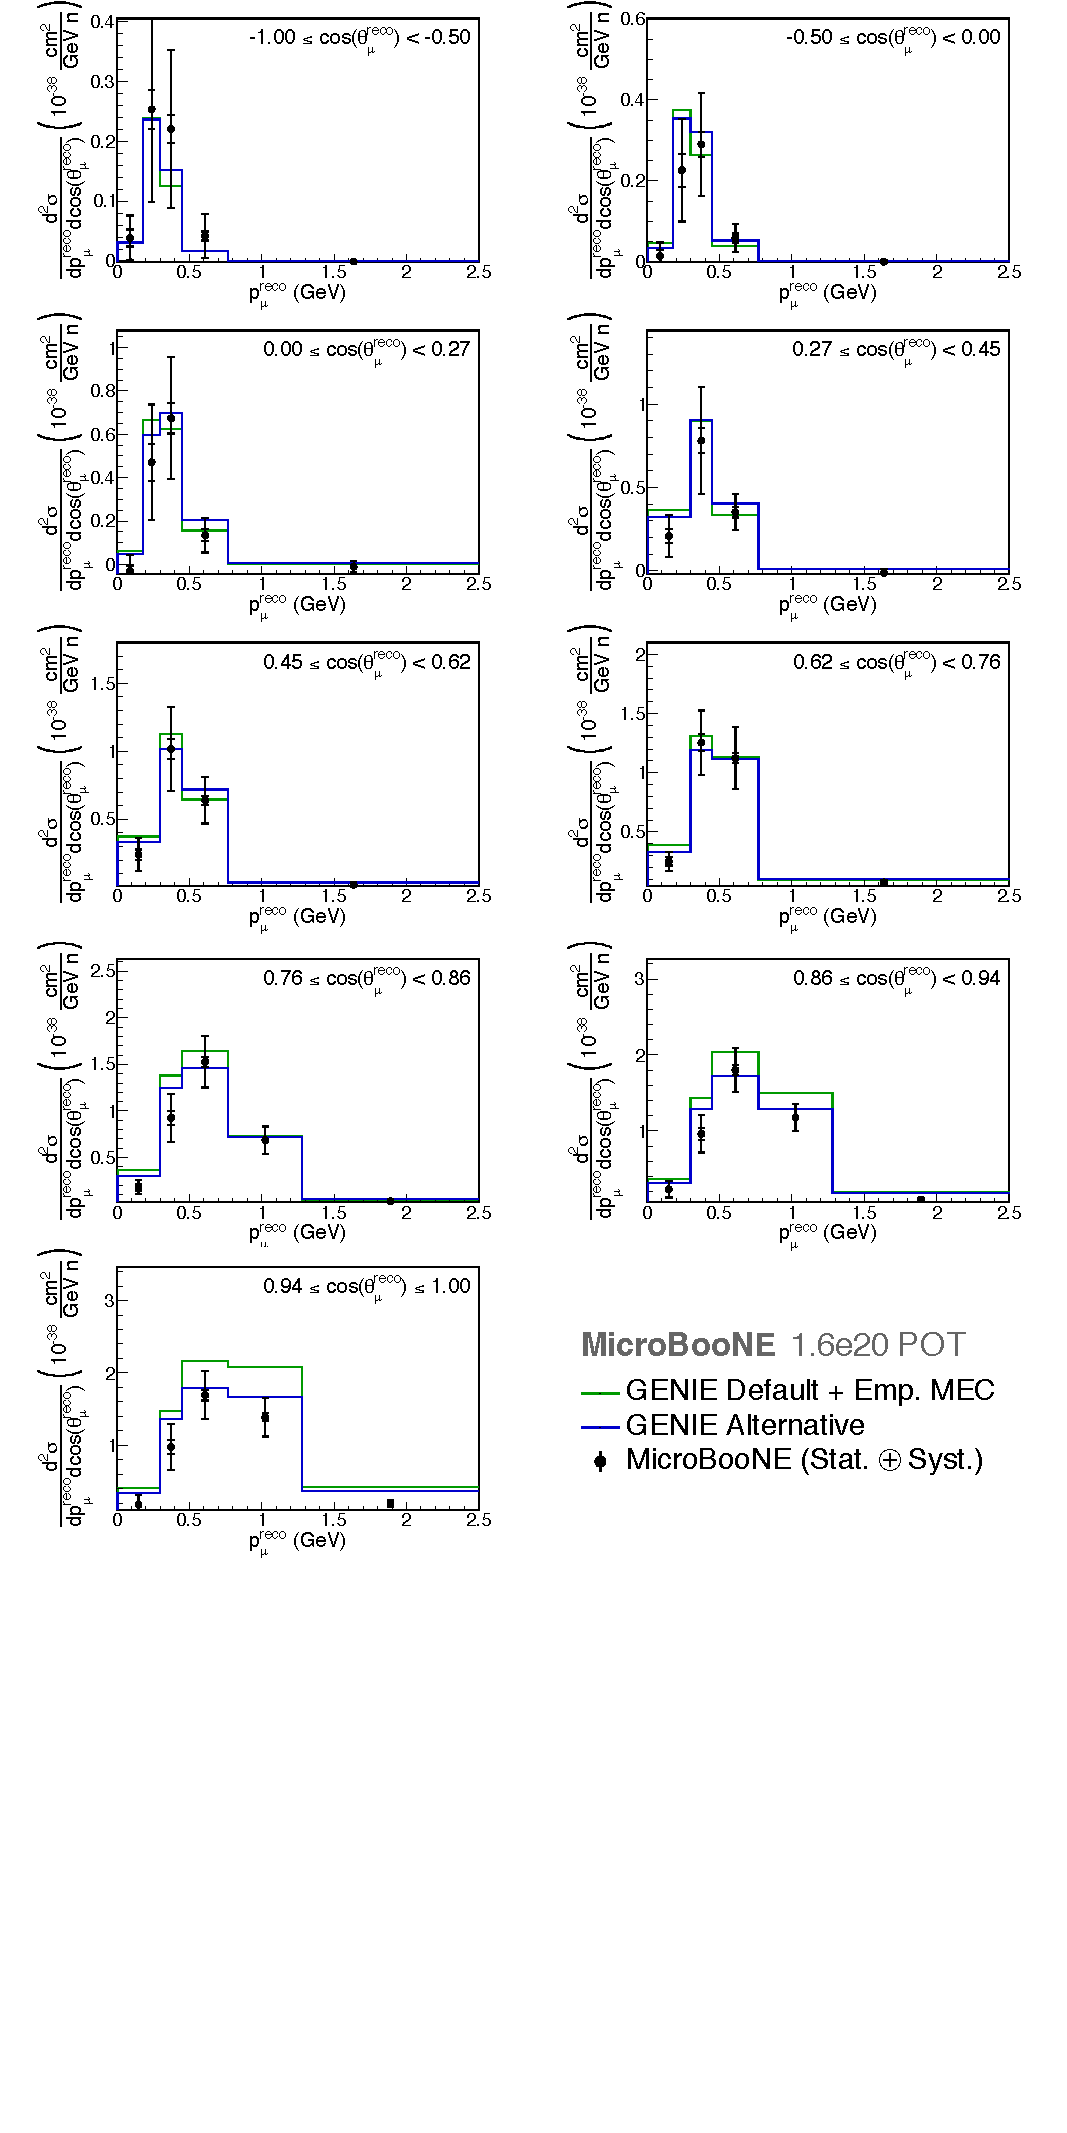
\includegraphics[width=.90\textwidth]{images/XSecFinal/xsec_bigger} %trkcostheta_trkmumom__xsec_anglesplit
\caption[Double-Differential Cross Section in $\cos\theta_\mu$ Bins (Stat. $\oplus$ Syst. Unc.)]{$\nu_\mu$ \acrshort{cc} inclusive double-differential cross section on argon per nucleon as a function of the reconstructed muon momentum and cosine of the reconstructed muon polar angle (angle with respect to the incoming neutrino direction). The data (black) is compared to the default \g prediction (green) and the alternative \g prediction (blue), as described in the text.  The inner vertical bars show statistical uncertainties, while the outer ones show the quadrature sum of the statistical and systematic uncertainties.}
\label{fig:trkcostheta_trkmumom__xsec_anglesplit}
\end{figure}

\begin{figure}[]
\begin{adjustwidth}{-1.3cm}{-1cm}
\centering
\subfloat[][Covariance matrix.]
   {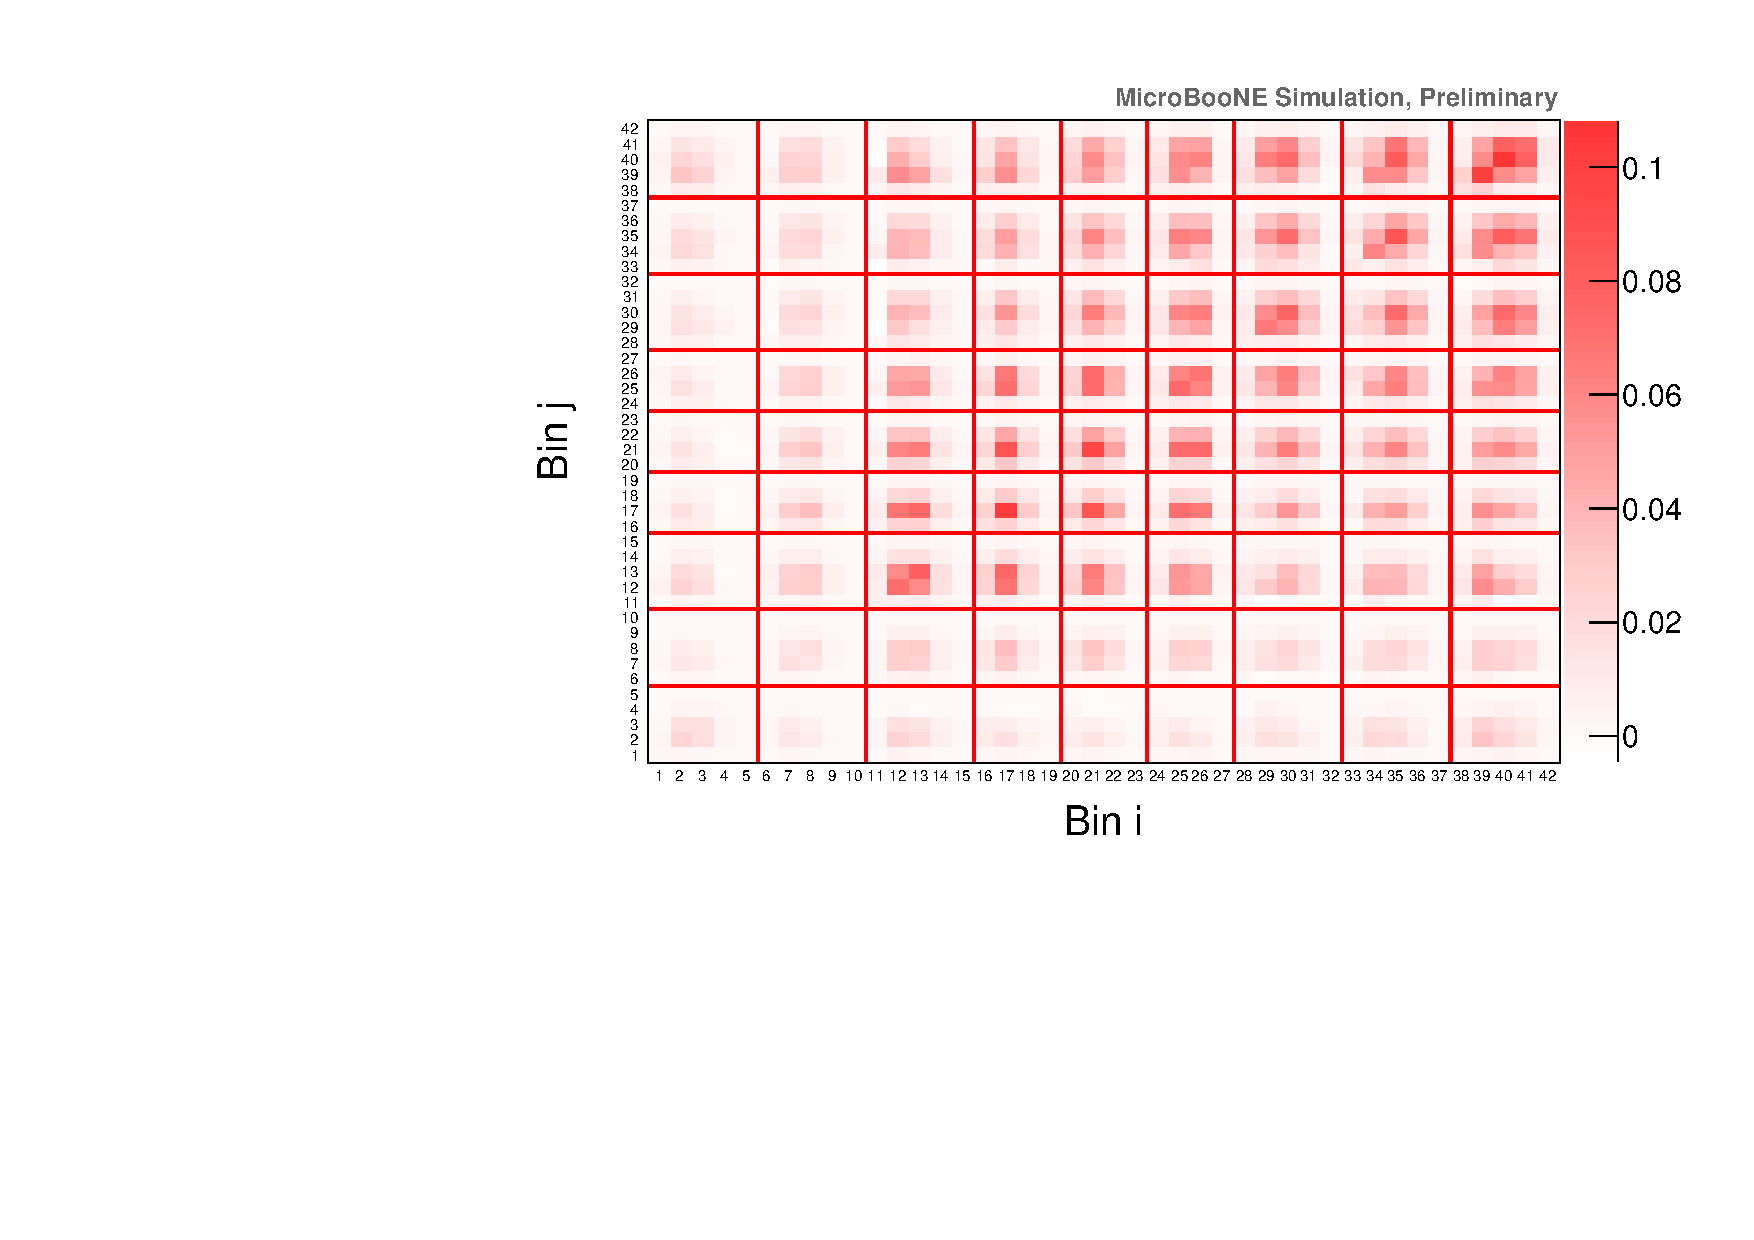
\includegraphics[width=.60\textwidth]{images/XSecFinal/trkcostheta_trkmumom__tot_covariance}
   \label{fig:trkcostheta_trkmumom__tot_covariance}} \quad
\subfloat[][Fractional covariance matrix.]
   {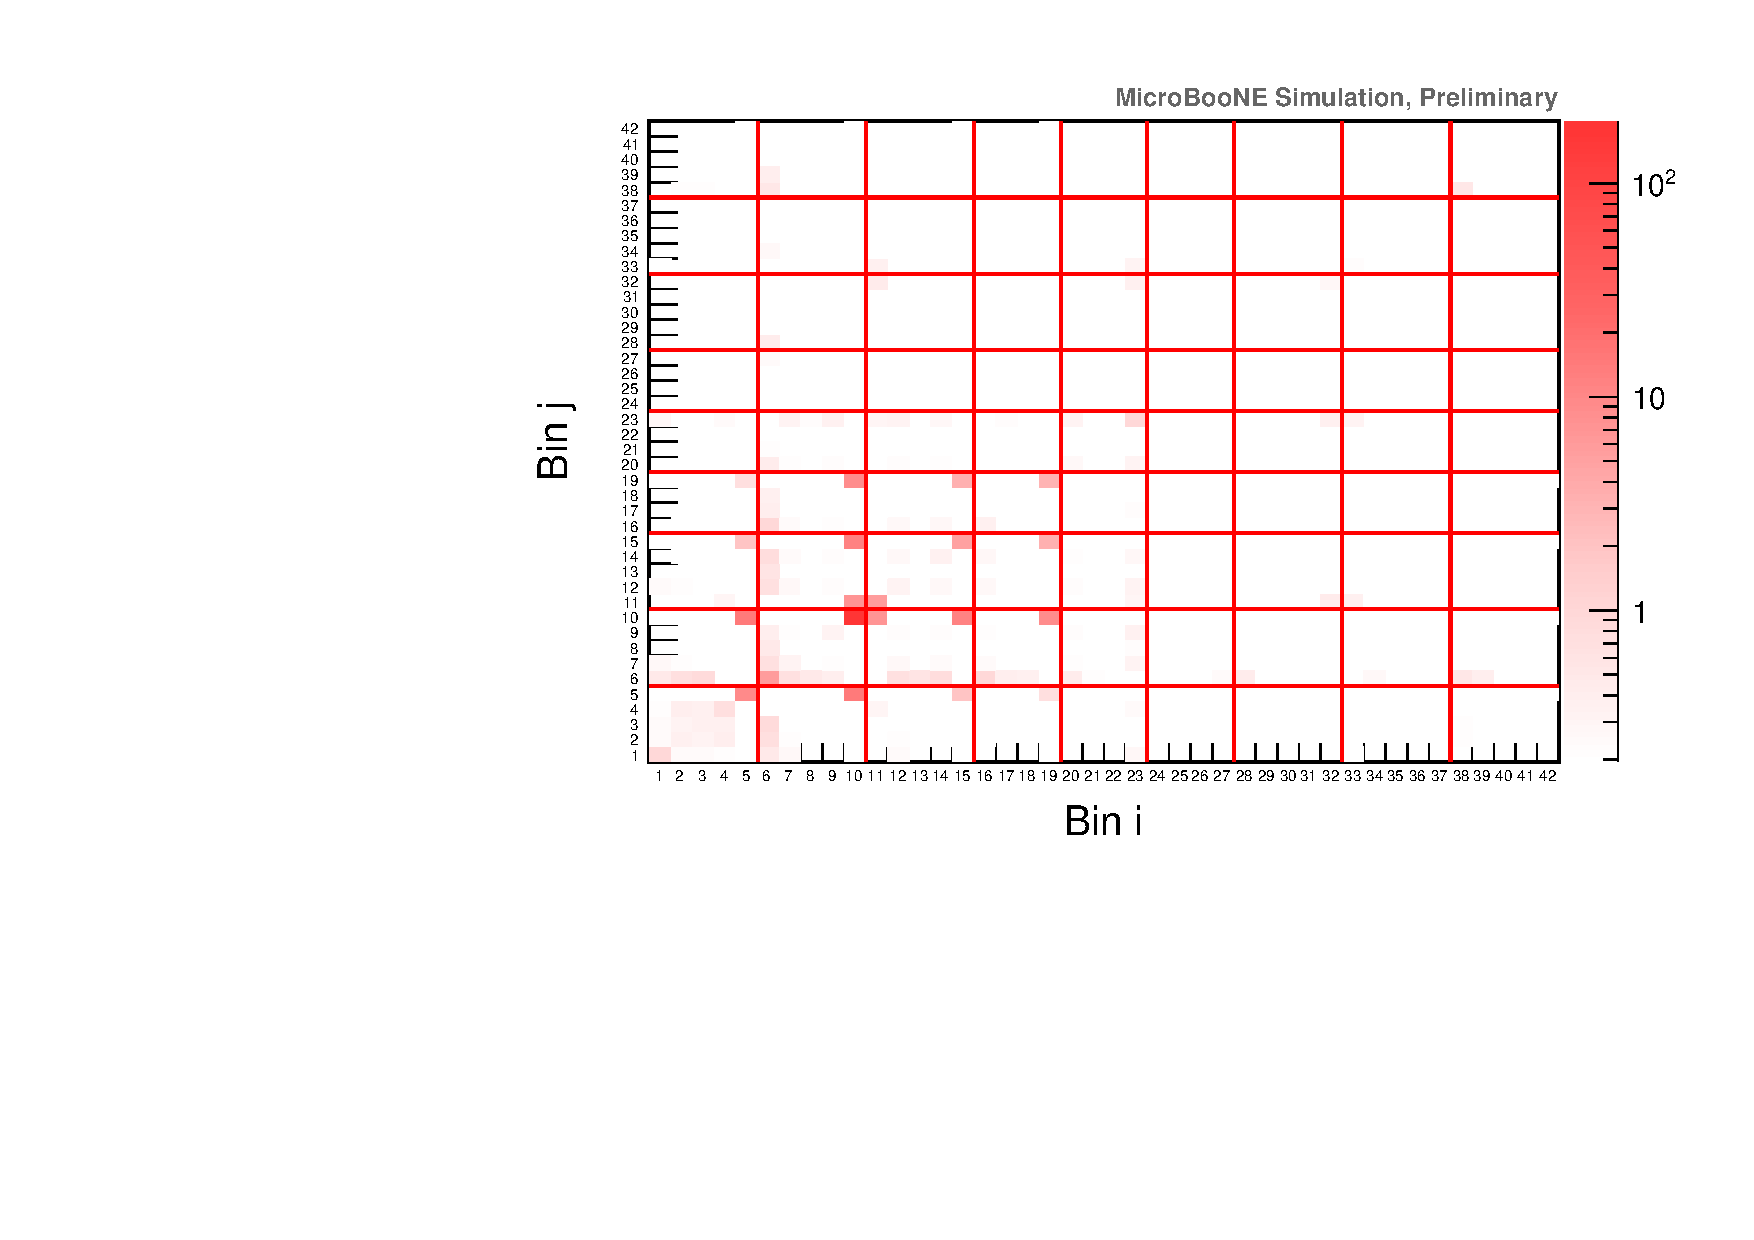
\includegraphics[width=.60\textwidth]{images/XSecFinal/trkcostheta_trkmumom__tot_fractional_covariance}
   \label{fig:trkcostheta_trkmumom__tot_fractional_covariance}} \quad
\subfloat[][Correlation matrix.]
   {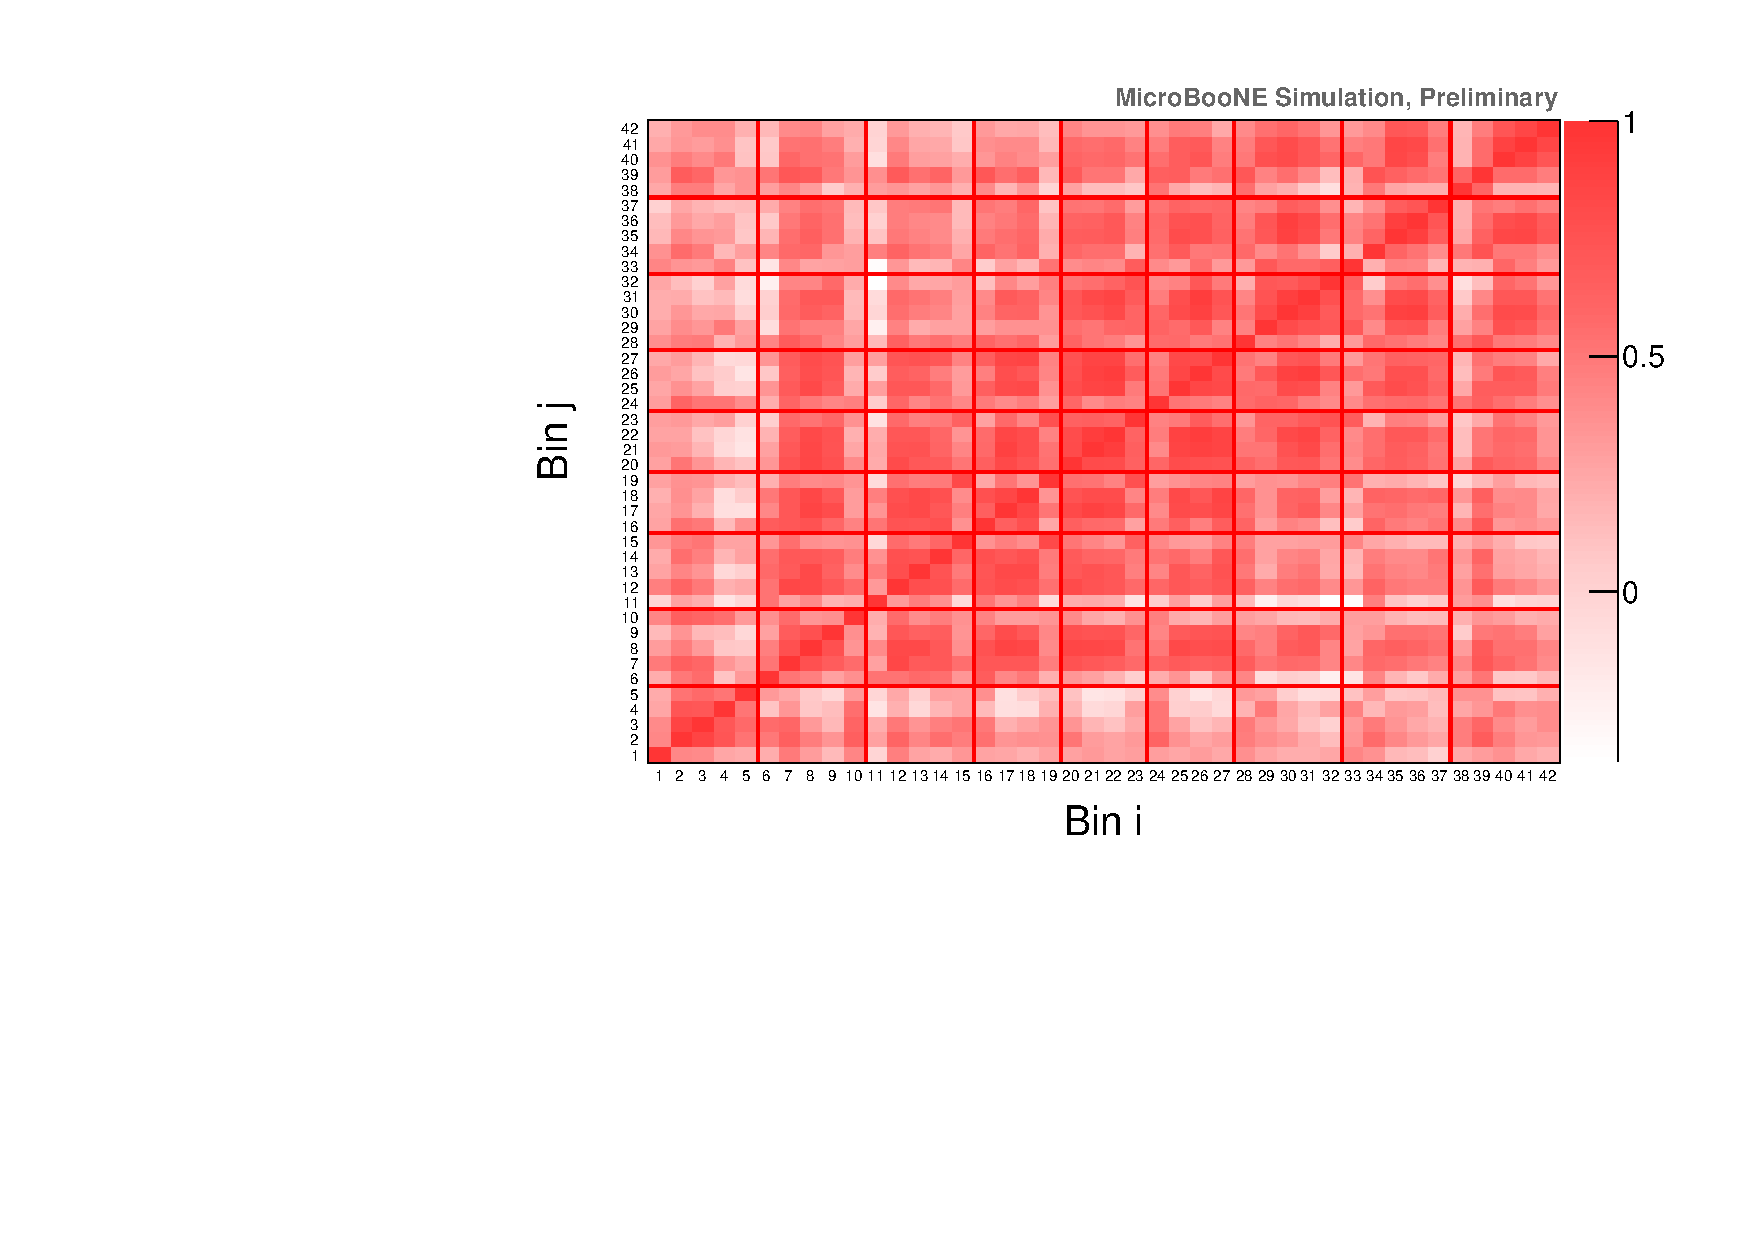
\includegraphics[width=.60\textwidth]{images/XSecFinal/trkcostheta_trkmumom__tot_correlation}
   \label{fig:trkcostheta_trkmumom__tot_correlation}} \\
\caption[Double-Differential Cross Section Total Covariance Matrix]{Total covariance~\protect\subref{fig:trkcostheta_trkmumom__tot_covariance}, fractional covariance~\protect\subref{fig:trkcostheta_trkmumom__tot_fractional_covariance} and correlation~\protect\subref{fig:trkcostheta_trkmumom__tot_correlation} matrices for the $(p_\mu, \cos\theta_\mu)$ bins. For the bin definition, see Section~\ref{sec:binning}.}
\label{fig:xsec_tot_correlation}
\end{adjustwidth}
\end{figure}



\clearpage

\section{Hypotheses Testing}
\label{sec:chi2}

In this Section, the two set of neutrino interaction models (``\tuneone'' and ``\tunethree'') will be quantitatively compared with the double differential cross-section measurement. A chi-squared $\chi^2$ test statistic is used assuming a multi-dimensional Gaussian approximation~\cite{cowan}:
\begin{equation}
\chi^2 = \sum_{ij} (x_i - \mu_i) \cdot E^{-1}_{ij} \cdot (x_j - \mu_j),
\end{equation}
where $x_{i(j)}$ is the measured double-differential cross section in bin $i(j)$, $\mu_{i(j)}$ is the predicted cross section in bin $i(j)$ and $E_{ij}$ is the total covariance matrix defined in Equation~\eqref{eq:tot_cov} and shown in Figure~\ref{fig:trkcostheta_trkmumom__tot_covariance}.
The measured $\chi^2$ under the \g default, $\chi^2_\text{def.}$, and alternative, $\chi^2_\text{alt.}$, are calculated:
\begin{equation}
\begin{split}
\chi^2_\text{def.} &= 246, \\
\chi^2_\text{alt.} &= 210.
\end{split}
\end{equation}
With 42 degrees of freedom, the $p$-values turn out to be extremely small ($\sim 2\times 10^{-30}$ and $\sim 5\times 10^{-24}$ respectively) which means both hypotheses can be rejected given the measured data and the estimated systematic uncertainties. 
%The discriminating power comes from the non-diagonal entries in the covariance matrix. 
The $\chi^2$ result is mainly driven by off-diagonal entries in the covariance matrix, especially in the detector systematic covariance matrix, for which the induced-charge is the dominant effect, as shown in Chapter~\ref{ch:systematics}. 
%This effect is currently being studied and the result will improve once a better modelling of the detector will be available.

Moreover, the measured data is also able to discriminate between the two models. This is shown by the difference between the $\chi^2$ calculated under the \g alternative and default hypotheses, resulting in
\begin{equation}
\Delta\chi^2 = \chi^2_\text{alt.} - \chi^2_\text{def.} = -36.8.
\end{equation}
To understand the statistical significance of this result, the expected distributions of the $\Delta\chi^2$ variable must be calculated. This can be done by using the Gaussian approximation as described in \cite{qian_original, qian}, where it is shown that the $\Delta\chi^2$ distribution can be approximated by a Gaussian with mean $\overline{\Delta\chi^2_\text{def.}} = \chi^2_\text{alt.}(x_\text{def.}^\text{Asimov})$ and standard deviation $2\sqrt{|\overline{\Delta\chi^2_\text{def.}}|}$ under \g default, and mean $\overline{\Delta\chi^2_\text{alt.}} = \chi^2_\text{def.}(x_\text{alt.}^\text{Asimov})$ and standard deviation $2\sqrt{|\overline{\Delta\chi^2_\text{alt.}}|}$ under \g alternative . Here, $x_\text{def.(alt.)}^\text{Asimov}$ is the Asimov dataset under \g default (alternative), which is taken to be the \g default (alternative) simulation itself.

The Asimov $\Delta\chi^2$ under the default and alternative hypotheses amounts to $\overline{\Delta\chi^2_\text{def.}} = 31.3$ and $\overline{\Delta\chi^2_\text{alt.}} = -30.9$, respectively. The $\Delta\chi^2$ expected distributions under the two hypotheses are shown in Figure~\ref{fig:chi2}. The two-side $p$-value is estimated to be $1.1 \times 10^{-9}$ under the default hypothesis, which in Gaussian standard deviation $\sigma$ gives more than a $6\sigma$ exclusion of the default model set. Also here the discriminating power comes from the non-diagonal entries in the covariance matrix, which do not allow much freedom for shape adjustments.

\begin{figure}[t]
\centering
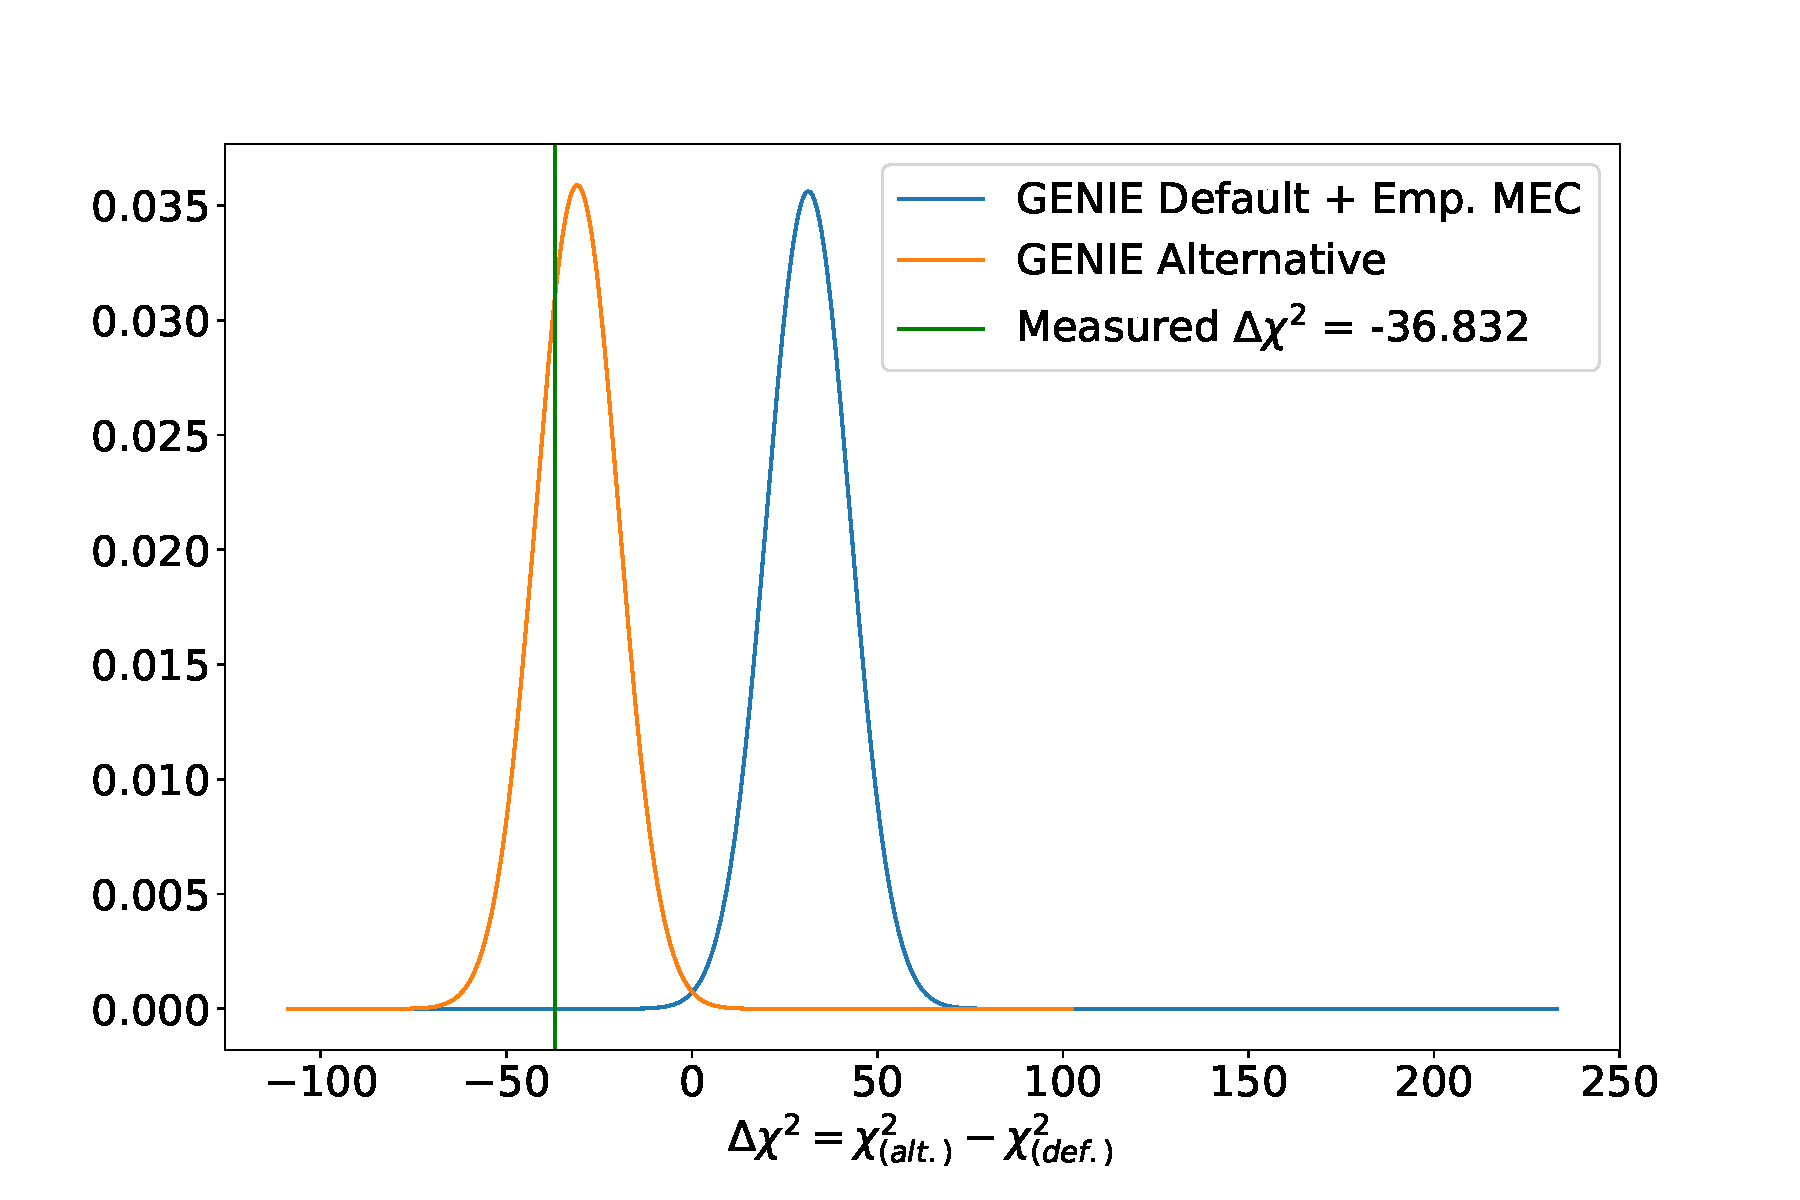
\includegraphics[width=.70\textwidth]{images/chi2}
\caption[$\Delta\chi^2$ Expected Distributions]{Expected distributions for $\Delta\chi^2 = \chi^2_\text{alt.} - \chi^2_\text{def.}$ under the ``\tuneone'' (blue) and ``\tunethree'' (orange) hypotheses. The measured delta chi-squared ($\Delta\chi^2 = -36.8$) is also shown with a green line.}
\label{fig:chi2}
\end{figure}


This result implies that the \g default model is excluded given the current data in favour of the alternative one. 
Statistics are highest in the most forward- going region of muon phase-space, where both the default and alternative model appear to over-predict the signal. This region is dominated by \acrshort{mec} events, and shows a stronger preference for the alternative model than the more \acrshort{qe} dominated regions. This is expected as the ``Valencia'' model folds interaction of correlated pairs and \acrshort{rpa} to describe many-body interactions into the calculation, versus an empirical correction to the \acrshort{cc} \acrshort{qe} events in the default configuration. Nevertheless, the measured cross section is slightly lower than the predicted \g cross section, even in the more theory-driven alternative \g configuration.












